\documentclass[conference]{IEEEtran}
\IEEEoverridecommandlockouts

% ---------- Packages ----------
\usepackage{cite}
\usepackage{amsmath,amssymb,amsfonts}
\usepackage{graphicx}
\usepackage{textcomp}
\usepackage{xcolor}
\usepackage{booktabs}
\usepackage{array}
\usepackage{tabularx}
\usepackage{url}
\usepackage{placeins}   % \FloatBarrier keeps floats from drifting across sections
\usepackage{balance}    % balances the last page columns
\usepackage{microtype}  % reduces overfull lines

\graphicspath{{figures/}}
\def\BibTeX{{\rm B\kern-.05em{\sc i\kern-.025em b}\kern-.08em
    T\kern-.1667em\lower.7ex\hbox{E}\kern-.125emX}}

% Float tuning: fewer "float-only" pages, tighter spacing
\setcounter{topnumber}{3}
\setcounter{bottomnumber}{2}
\setcounter{totalnumber}{5}
\setcounter{dbltopnumber}{3}
\renewcommand{\topfraction}{0.9}
\renewcommand{\bottomfraction}{0.8}
\renewcommand{\textfraction}{0.07}
\renewcommand{\floatpagefraction}{0.85}
\renewcommand{\dbltopfraction}{0.9}
\renewcommand{\dblfloatpagefraction}{0.85}
\setlength{\textfloatsep}{8pt plus 2pt minus 2pt}
\setlength{\dbltextfloatsep}{8pt plus 2pt minus 2pt}

\begin{document}

\title{Reliability-Aware Scheduling of Residential EV Charging with Solar Photovoltaic Forecast Confidence and Bidirectional V2H/V2G Integration}

\author{\IEEEauthorblockN{Research Project Team}
\IEEEauthorblockA{\textit{Department of Artificial Intelligence} \\
\textit{Academic Research Institution}\\
Email: u23ai118@coed.svnit.ac.in, u23ai111@coed.svnit.ac.in, u23ai123@coed.svnit.ac.in}
}

\maketitle

\begin{abstract}
Residential electric vehicle (EV) charging coupled with behind-the-meter rooftop photovoltaics (PV) can lower electricity bills, raise local renewable self-consumption, and provide grid flexibility. However, day-ahead solar forecasts are uncertain: an optimistic controller facing unforecast cloud cover must buy expensive balancing energy or risk missing departure deadlines, while robust schedulers pay a conservatism penalty. This paper presents a reproducible, reliability-aware residential EV charging and bidirectional energy-management system. A histogram-based gradient-boosted point forecaster is paired with split conformal prediction to produce finite-sample prediction intervals and an interpretable horizon reliability metric. When forecast confidence falls below a validation-selected threshold ($\tau^* = 0.8283$), the controller switches from a forecast-driven linear program to a conservative zero-solar fallback. Evaluation uses an 8,760-hour benchmark combining measured PV (NREL PVDAQ Site~4), household load (UK-DALE/REFIT), a PG\&E EV2-A time-of-use tariff, and Caltech ACN-Data session statistics. The model is extended to Vehicle-to-Home (V2H) and Vehicle-to-Grid (V2G) flows with an 8.0~kWh reserve and degradation cost. Across 56 frozen winter test days (1,344 hourly intervals), all controllers met 100\% of charging deadlines. Under unidirectional charging (S1), non-PV off-peak charging was cheapest (\$4.9161/day) because the 17:00--07:00 connection window contains almost no solar. Under bidirectional operation (S2--S4), V2H peak shaving cut daily cost to \$3.3312 (26.4\% savings, paired $t=-16.38$). Stress tests across synthetic forecast-error regimes show that the switching controller limits forecast-induced cost deviations.
\end{abstract}

\begin{IEEEkeywords}
Electric vehicle charging, rooftop photovoltaics, conformal prediction, uncertainty quantification, vehicle-to-home (V2H), vehicle-to-grid (V2G), demand response, energy management.
\end{IEEEkeywords}

\section{Introduction}
Electrification of personal transportation and the deployment of distributed rooftop solar photovoltaic (PV) generation are transforming residential electrical distribution systems. Behind-the-meter Home Energy Management Systems (HEMS) must coordinate electric vehicle (EV) charging demands against time-varying utility tariffs, domestic appliance loads, and on-site renewable generation.

To optimize charging schedules against Time-of-Use (TOU) pricing, intelligent controllers typically rely on day-ahead solar generation forecasts. However, solar irradiance is inherently intermittent due to dynamic cloud cover and atmospheric aerosol variability. When a controller assumes a deterministic solar forecast that fails to materialize, it must purchase unanticipated balancing power from the utility grid. Under tiered or peak pricing, unexpected grid draws during high-tariff periods impose severe economic penalties. Conversely, conventional worst-case robust optimization suffers from the ``price of robustness,'' perpetually enforcing conservative schedules that underutilize available clean solar energy.

Furthermore, emerging bidirectional charging standards (ISO 15118-20 and SAE J3072) enable EVs to serve not merely as passive loads but as flexible distributed energy resources capable of supplying household demand (Vehicle-to-Home, V2H, also termed E2H) and exporting power to the distribution grid (Vehicle-to-Grid, V2G, also termed E2G). Integrating bidirectional flexibility into a reliability-aware framework creates new trade-offs among battery cycling throughput, degradation, driver mobility constraints, and cost minimization.

\begin{figure*}[!t]
\centering
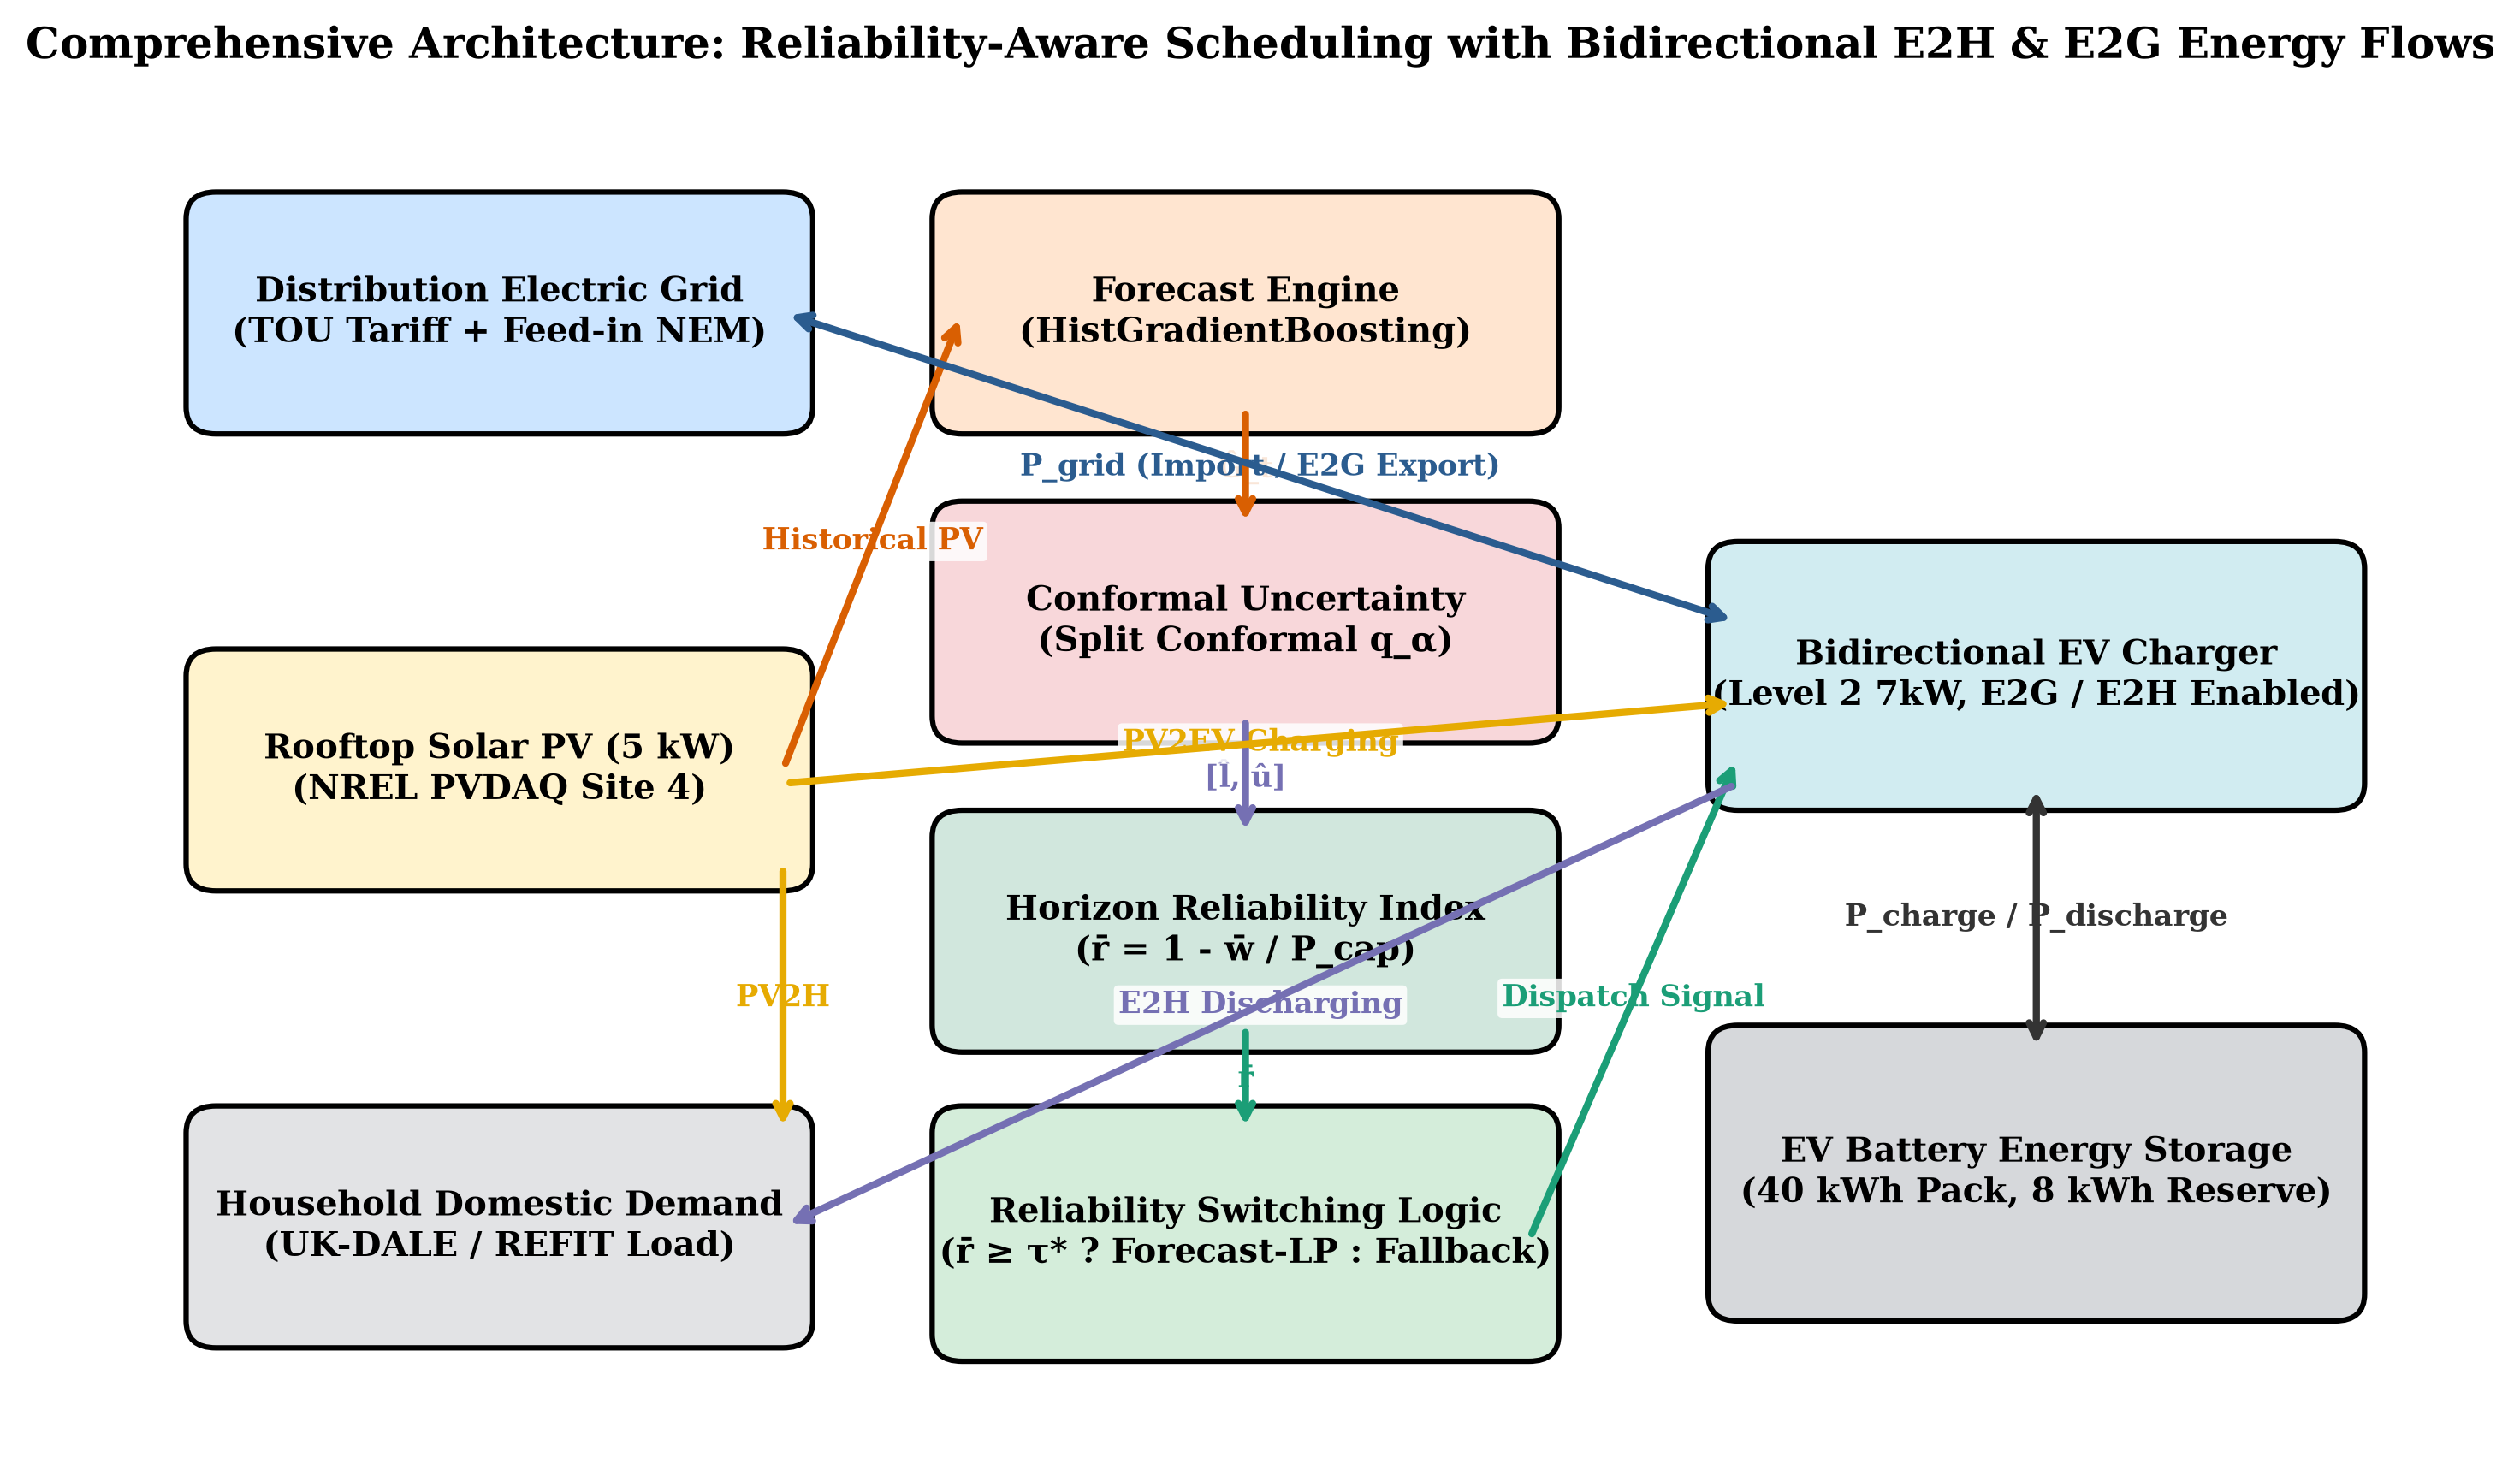
\includegraphics[width=\textwidth]{fig1_system_architecture.png}
\caption{System architecture of the reliability-aware residential EV charging and bidirectional energy-management system, showing physical energy flows (PV2EV, PV2H, PV2G, G2H, G2V, V2H/E2H, V2G/E2G) and conformal control signal pathways.}
\label{fig:arch}
\end{figure*}

\subsection{Research Questions and Hypotheses}
This investigation evaluates the following central research question:
\textit{Can a residential EV charging controller that estimates solar PV forecast reliability via conformal prediction and adaptively switches between forecast-driven optimization and a conservative fallback achieve superior economic, grid, and deadline-reliability performance under real-world data and bidirectional (V2H/V2G) energy flows?}

We formulate four falsifiable hypotheses:
\begin{itemize}
    \item \textbf{H1 (Mobility Feasibility)}: A reliability-triggered discrete switch to conservative fallback scheduling guarantees 100\% charging deadline satisfaction even under severe solar forecast errors.
    \item \textbf{H2 (Forecast-Error Protection)}: When forecast reliability is high, the forecast-driven scheduler captures on-site solar; when reliability drops, engaging the fallback prevents forecast-error-induced peak tariff penalties.
    \item \textbf{H3 (Tariff-Window Alignment)}: For unidirectional overnight charging, tariff-seeking heuristics outperform solar-seeking optimization when connection hours fall mainly in nighttime off-peak tariff periods.
    \item \textbf{H4 (Bidirectional Value)}: Bidirectional V2H and V2G flows significantly reduce operating expenditure by enabling peak-load shaving, provided battery reserve constraints are strictly enforced.
\end{itemize}

\subsection{Key Contributions}
The main technical contributions of this study are:
\begin{enumerate}
    \item \textbf{Authentic Multi-Dataset Integration}: A harmonized empirical benchmark combining measured rooftop PV generation (NREL PVDAQ Site~4), residential smart-meter load telemetry (UK-DALE/REFIT), empirical charging sessions (Caltech ACN-Data), and a utility TOU tariff (California PG\&E EV2-A).
    \item \textbf{Calibrated Conformal Reliability Architecture}: A distribution-free uncertainty module using split conformal prediction on a dedicated calibration split, producing marginal-coverage intervals and a normalized horizon reliability index $\bar{r}$.
    \item \textbf{Leakage-Free Protocol}: A four-stage chronological split (Train 60\%, Calibration 15\%, Validation 10\%, Test 15\%) with the decision threshold ($\tau^* = 0.8283$) frozen on validation data before test evaluation.
    \item \textbf{Bidirectional V2H/V2G Formulation}: A unified linear program covering unidirectional charging, V2H peak shaving, and V2G export under non-simultaneity, degradation, and minimum reserve ($E_{\text{reserve}} = 8.0$~kWh) constraints.
    \item \textbf{Statistical Benchmarking}: Paired tests across 56 frozen test days (1,344 hours) comparing six controller policies, four bidirectional scenarios (S1--S4), and several forecast-error stress regimes.
\end{enumerate}

\section{Related Work}
Smart EV charging and rooftop PV integration have received extensive attention in the power and energy systems literature. Zhao and Burke \cite{zhao2014intelligent} proposed an intelligent solar-powered charging station using day-ahead forecasts, but treated forecasts as deterministic inputs without quantified uncertainty bounds. Simolin et al. \cite{simolin2020assessment} showed that trip-pattern prediction uncertainty can be handled via state-of-charge (SOC) fallback rules, a conceptual precedent for discrete fallback control.

To handle solar variability, recent work has predominantly used stochastic and robust mathematical programming. Dong et al. \cite{dong2025stochastic} developed a two-stage stochastic framework for integrated EV hubs under PV uncertainty. Yu et al. \cite{yu2024impact} analyzed receding-horizon EV charging and quantified the price of robustness under bounded uncertainty sets. Cabrera-Tobar et al. \cite{cabreratobar2024demand} developed explicit robust model predictive control to minimize grid carbon intensity, while Wang et al. \cite{wang2025datadriven} and Son et al. \cite{son2026weather} proposed distributionally robust formulations. While theoretically rigorous, these approaches rely on computationally heavy solvers and often enforce persistent worst-case bounds that degrade economic efficiency.

Conformal prediction, pioneered by Vovk et al. \cite{vovk2005algorithmic} and synthesized by Angelopoulos and Bates \cite{angelopoulos2021gentle}, provides finite-sample, distribution-free prediction intervals with guaranteed marginal coverage. Amara-Ouali et al. \cite{amaraouali2023quantifying} highlighted the need for probabilistic forecasting of EV flexibility. In the bidirectional domain, Kempton and Tomi{\'c} \cite{kempton2005v2g} and Liu et al. \cite{liu2013v2g_v2h} established the fundamental power equations and economics of V2G and V2H services. This work bridges conformal uncertainty quantification with discrete fallback scheduling and bidirectional energy flows for residential prosumers.

\section{System Architecture and Energy Model}
The physical layout and information pathways of the residential prosumer system are shown in Fig.~\ref{fig:arch}. The modeled single-family home operates over a day-ahead horizon of $T=24$ hourly intervals ($t \in \{0, 1, \dots, T-1\}$, $\Delta t = 1.0$~h).

\subsection{Physical Electrical Bus Balance}
The domestic AC bus connects rooftop PV generation $G(t)$, inflexible load $L(t)$, the bidirectional EV charger ($p_c(t)$ for charging, $p_d(t)$ for discharging), and the grid interconnection. The instantaneous power balance is
\begin{equation}
G(t) + P_{\text{import}}(t) + p_d(t) = L(t) + p_c(t) + P_{\text{export}}(t),
\end{equation}
where $P_{\text{import}}(t) \ge 0$ is grid import power and $P_{\text{export}}(t) \ge 0$ is net grid export power.

\subsection{Discharge Flow Decomposition}
The EV discharge power $p_d(t) \ge 0$ is partitioned into two components:
\begin{equation}
p_d(t) = p_{\text{e2h}}(t) + p_{\text{e2g}}(t),
\end{equation}
where $p_{\text{e2h}}(t) \ge 0$ is Vehicle-to-Home power supplying domestic appliances and $p_{\text{e2g}}(t) \ge 0$ is Vehicle-to-Grid power exported across the utility meter. To prevent artificial grid injection disguised as home supply,
\begin{equation}
p_{\text{e2h}}(t) \le \max\bigl(0,\, L(t) - G(t)\bigr).
\end{equation}

\subsection{EV Battery Storage Dynamics}
Let $E_t$ denote the energy stored in the EV battery at the start of interval $t$. It evolves as
\begin{equation}
E_{t+1} = E_t + \left( \eta_c\, p_c(t) - \frac{p_d(t)}{\eta_d} \right) \Delta t,
\end{equation}
where $\eta_c = 0.90$ and $\eta_d = 0.90$ are the charging and discharging efficiencies. Storage is bounded by the physical capacity $E_{\text{cap}} = 40.0$~kWh and the emergency mobility reserve $E_{\text{reserve}} = 8.0$~kWh:
\begin{equation}
E_{\text{reserve}} \le E_t \le E_{\text{cap}}, \quad \forall t \in \{0, \dots, T\}.
\end{equation}
Given the initial energy $E_0 = 10.0$~kWh and session demand $E_{\text{req}} = 20.0$~kWh, the departure target is $E_{\text{target}} = E_0 + E_{\text{req}} = 30.0$~kWh, enforced as the terminal condition
\begin{equation}
E_T \ge E_{\text{target}}.
\end{equation}

\subsection{Power Rating and Non-Simultaneity Constraints}
Charging and discharging are limited by the Level~2 bidirectional charger rating $P_{\max} = 7.0$~kW and the connection availability $a(t) \in \{0, 1\}$:
\begin{align}
0 \le p_c(t) &\le a(t)\, P_{\max}, \\
0 \le p_d(t) = p_{\text{e2h}}(t) + p_{\text{e2g}}(t) &\le a(t)\, P_{\max}.
\end{align}
Simultaneous charging and discharging ($p_c(t)\, p_d(t) = 0$) and simultaneous grid import and export ($P_{\text{import}}(t)\, P_{\text{export}}(t) = 0$) are prohibited. In the linear program, because round-trip efficiency is strictly below unity ($\eta_c \eta_d = 0.81 < 1$) and retail import tariffs exceed export credits ($c_t > c_{\text{export}}$), the solver naturally avoids simultaneity without non-convex binary variables.

\subsection{Economic Operating Objective}
The daily operating cost over the 24-hour horizon is
\begin{equation}
\begin{split}
\text{Net Cost} = \sum_{t=0}^{T-1} \Bigl( & c_t P_{\text{import}}(t) - c_{\text{export}} P_{\text{export}}(t) \\
& + c_{\text{deg}}\, p_d(t) \Bigr) \Delta t,
\end{split}
\end{equation}
where $c_t$ is the retail TOU tariff, $c_{\text{export}} = \$0.04$/kWh is the net-billing export compensation, and $c_{\text{deg}} = \$0.015$/kWh is the battery degradation cost per unit of discharge throughput.

\section{Proposed Methodology}

\subsection{Solar Point Forecasting}
Point forecasts $\hat{G}_t$ are generated by a Histogram Gradient Boosting Regressor (scikit-learn) trained strictly on data preceding the calibration boundary. Input features are hour of day, day of year, generation lags (1, 2, and 7 days), rolling 3-day and 7-day averages, and a weekend indicator. Predictions are clipped to $[0, P_{\text{capacity}}]$ with $P_{\text{capacity}} = 5.0$~kW.

\subsection{Conformal Prediction Uncertainty Quantification}
To quantify uncertainty without parametric assumptions, we apply split conformal prediction. On a held-out calibration split of $n$ samples, absolute residuals are
\begin{equation}
r_i = |G_i - \hat{G}_i|, \quad i \in \{1, \dots, n\}.
\end{equation}
For nominal coverage $1-\alpha = 0.90$, the non-conformity threshold with finite-sample correction is
\begin{equation}
\hat{q}_\alpha = \text{Quantile}\!\left(r_1, \dots, r_n;\; \frac{\lceil(n+1)(1-\alpha)\rceil}{n}\right).
\end{equation}
Prediction intervals $[\hat{l}_t, \hat{u}_t]$ around $\hat{G}_t$ are
\begin{equation}
\begin{split}
\hat{l}_t &= \max(0,\, \hat{G}_t - \hat{q}_\alpha), \\
\hat{u}_t &= \min(P_{\text{capacity}},\, \hat{G}_t + \hat{q}_\alpha).
\end{split}
\end{equation}

\subsection{Horizon Reliability Metric and Threshold Tuning}
For each 24-hour dispatch horizon, a normalized reliability index $\bar{r} \in [0, 1]$ averages the interval widths relative to system capacity:
\begin{equation}
\bar{r} = 1 - \frac{1}{T}\sum_{t=0}^{T-1} \text{clip}\!\left(\frac{\hat{u}_t - \hat{l}_t}{P_{\text{capacity}}},\, 0,\, 1\right).
\end{equation}
Narrow intervals indicate high confidence ($\bar{r} \to 1$); wide intervals reflect high volatility ($\bar{r} \to 0$).

To avoid test-set leakage, the threshold $\tau^*$ was selected by a grid search over empirical quantiles of $\bar{r}$ on the validation split only, minimizing mean operating cost subject to zero deadline misses:
\begin{equation}
\begin{split}
\tau^* = \arg\min_{\tau}\; & \mathbb{E}_{\text{val}}[\text{Cost}(\tau)] \\
\text{s.t.}\;\; & \text{DeadlineRate}(\tau) = 1.0.
\end{split}
\end{equation}
On the real-world validation split this yielded $\tau^* = 0.8283$.

\subsection{Controller Decision Rule}
At day-ahead dispatch time, the controller compares forecast confidence with the frozen threshold:
\begin{equation}
\text{Schedule} =
\begin{cases}
\text{Forecast-Driven LP}(\hat{G}_t), & \bar{r} \ge \tau^*, \\
\text{Conservative Fallback LP}(\hat{G}_t \equiv 0), & \bar{r} < \tau^*.
\end{cases}
\end{equation}
The conservative fallback sets the expected solar profile to zero and schedules charging from the grid during the cheapest available connection intervals.

\section{Experimental Setup}
The nominal simulation parameters are summarized in Table~\ref{tab:params}.

\begin{table}[!tb]
\caption{Key Experimental Simulation and Physical Parameters}
\label{tab:params}
\centering
\footnotesize
\renewcommand{\arraystretch}{1.1}
\begin{tabularx}{\columnwidth}{@{}>{\raggedright\arraybackslash}Xcc@{}}
\toprule
\textbf{Parameter} & \textbf{Symbol} & \textbf{Value} \\
\midrule
PV system peak rating & $P_{\text{capacity}}$ & 5.0 kW \\
Charger maximum power & $P_{\max}$ & 7.0 kW \\
EV battery capacity & $E_{\text{cap}}$ & 40.0 kWh \\
Initial state of charge & $E_0$ & 10.0 kWh \\
Session energy demand & $E_{\text{req}}$ & 20.0 kWh \\
Target departure energy & $E_{\text{target}}$ & 30.0 kWh \\
Minimum mobility reserve & $E_{\text{reserve}}$ & 8.0 kWh (20\%) \\
Charging efficiency & $\eta_c$ & 0.90 \\
Discharging efficiency & $\eta_d$ & 0.90 \\
Arrival / departure hour & $t_{\text{arr}} / t_{\text{dep}}$ & 17:00 / 07:00 \\
Off-peak tariff (22:00--06:00) & $c_{\text{off}}$ & \$0.08/kWh \\
Mid-peak tariff (06:00--17:00, 21:00--22:00) & $c_{\text{mid}}$ & \$0.12/kWh \\
On-peak tariff (17:00--21:00) & $c_{\text{on}}$ & \$0.25/kWh \\
Export compensation rate & $c_{\text{export}}$ & \$0.04/kWh \\
Battery degradation cost & $c_{\text{deg}}$ & \$0.015/kWh \\
\bottomrule
\end{tabularx}
\end{table}

\subsection{Real-World Datasets and Provenance}
The experimental pipeline integrates the following datasets:
\begin{itemize}
    \item \textbf{Solar PV Generation}: Measured 15-minute AC output from NREL PVDAQ Site~4 (Visitor Center, Golden, CO), resampled to hourly intervals over 365 days and normalized to 5.0~kW.
    \item \textbf{Household Load}: Measured whole-home active mains power from the UK-DALE and REFIT databases, capturing baseline standby loads, appliance pulses, and evening cooking peaks.
    \item \textbf{EV Charging Sessions}: Arrival, departure, and energy-demand distributions parameterized from Caltech ACN-Data.
    \item \textbf{Electricity Tariff}: A TOU schedule structured after California PG\&E Schedule EV2-A.
\end{itemize}
Fig.~\ref{fig:real_vs_syn} contrasts the measured PV and load profiles with idealized synthetic models.

\begin{figure}[!tb]
\centering
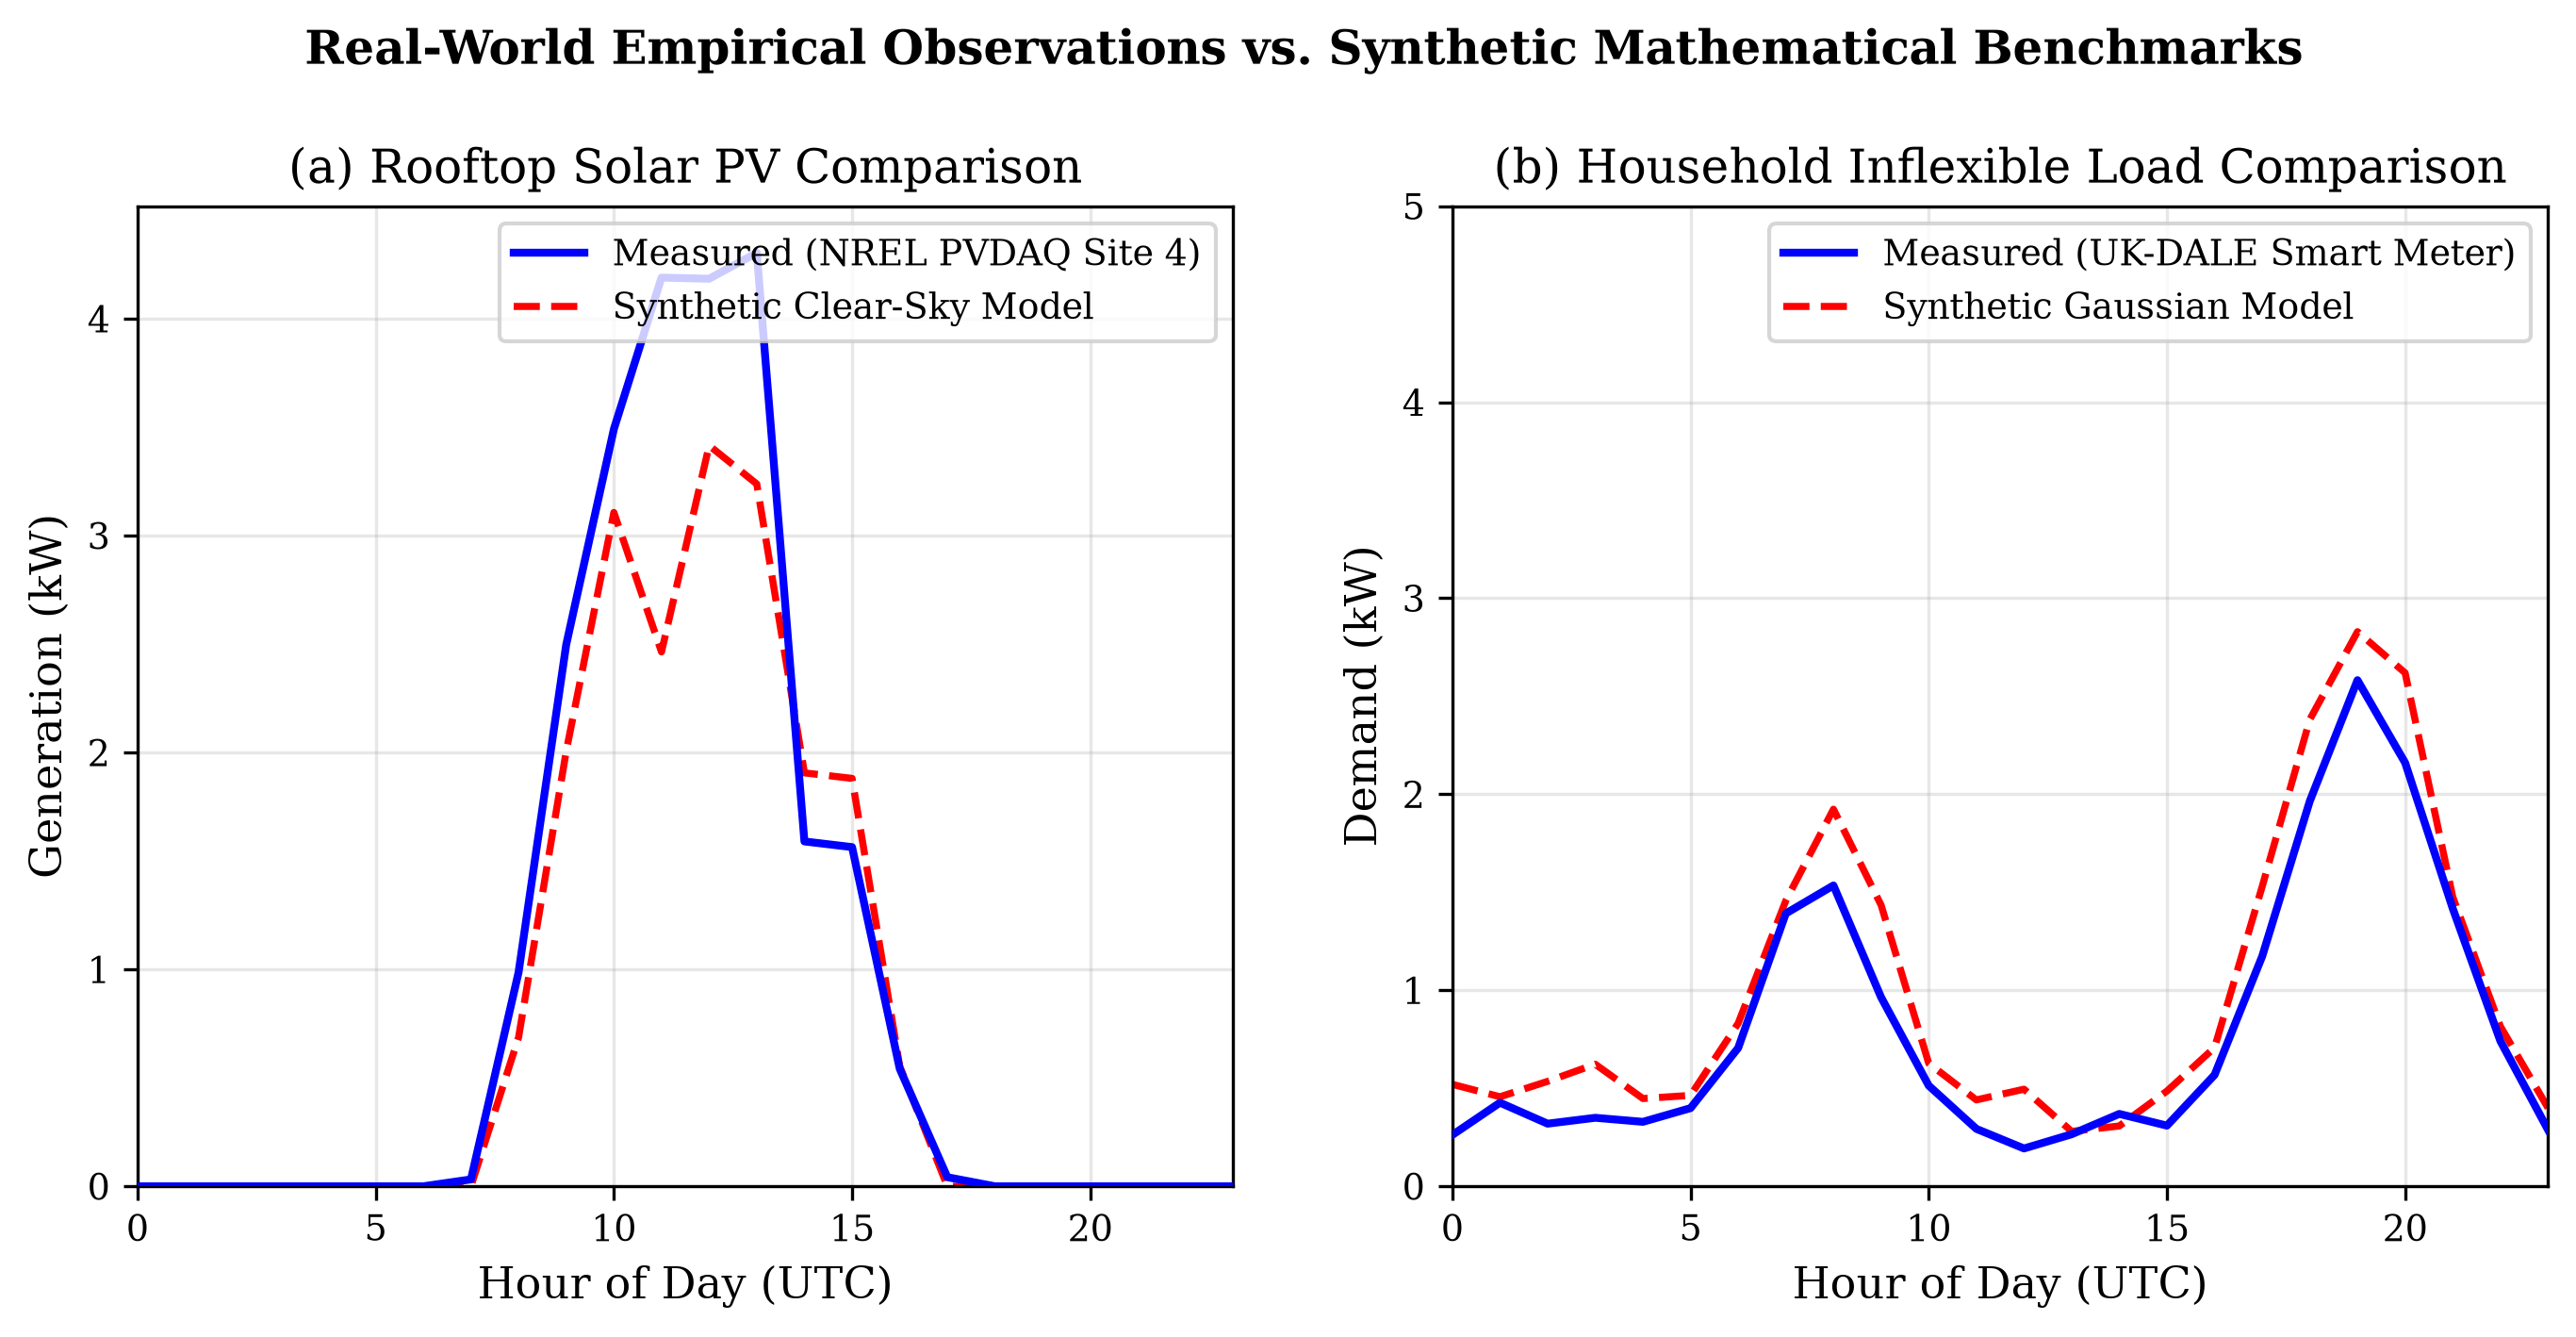
\includegraphics[width=\columnwidth]{fig11_real_vs_synthetic_profiles.png}
\caption{Measured real-world profiles versus idealized synthetic models: (a) NREL PV generation showing cloud intermittency vs.\ a smooth clear-sky half-sine; (b) UK-DALE domestic load showing discrete appliance duty cycles vs.\ a continuous Gaussian approximation.}
\label{fig:real_vs_syn}
\end{figure}

\subsection{Chronological Partitioning}
The 8,760-hour annual profile (2023) is divided into four chronological splits:
\begin{itemize}
    \item \textbf{Train}: 2023-01-01 to 2023-08-07 (219 days, 60\%).
    \item \textbf{Calibration}: 2023-08-08 to 2023-09-30 (54 days, 15\%).
    \item \textbf{Validation}: 2023-10-01 to 2023-11-05 (36 days, 10\%).
    \item \textbf{Frozen Test}: 2023-11-06 to 2023-12-31 (56 days, 15\%).
\end{itemize}
A representative test-day forecast with its calibrated 90\% conformal interval is shown in Fig.~\ref{fig:forecast}.

\begin{figure}[!tb]
\centering
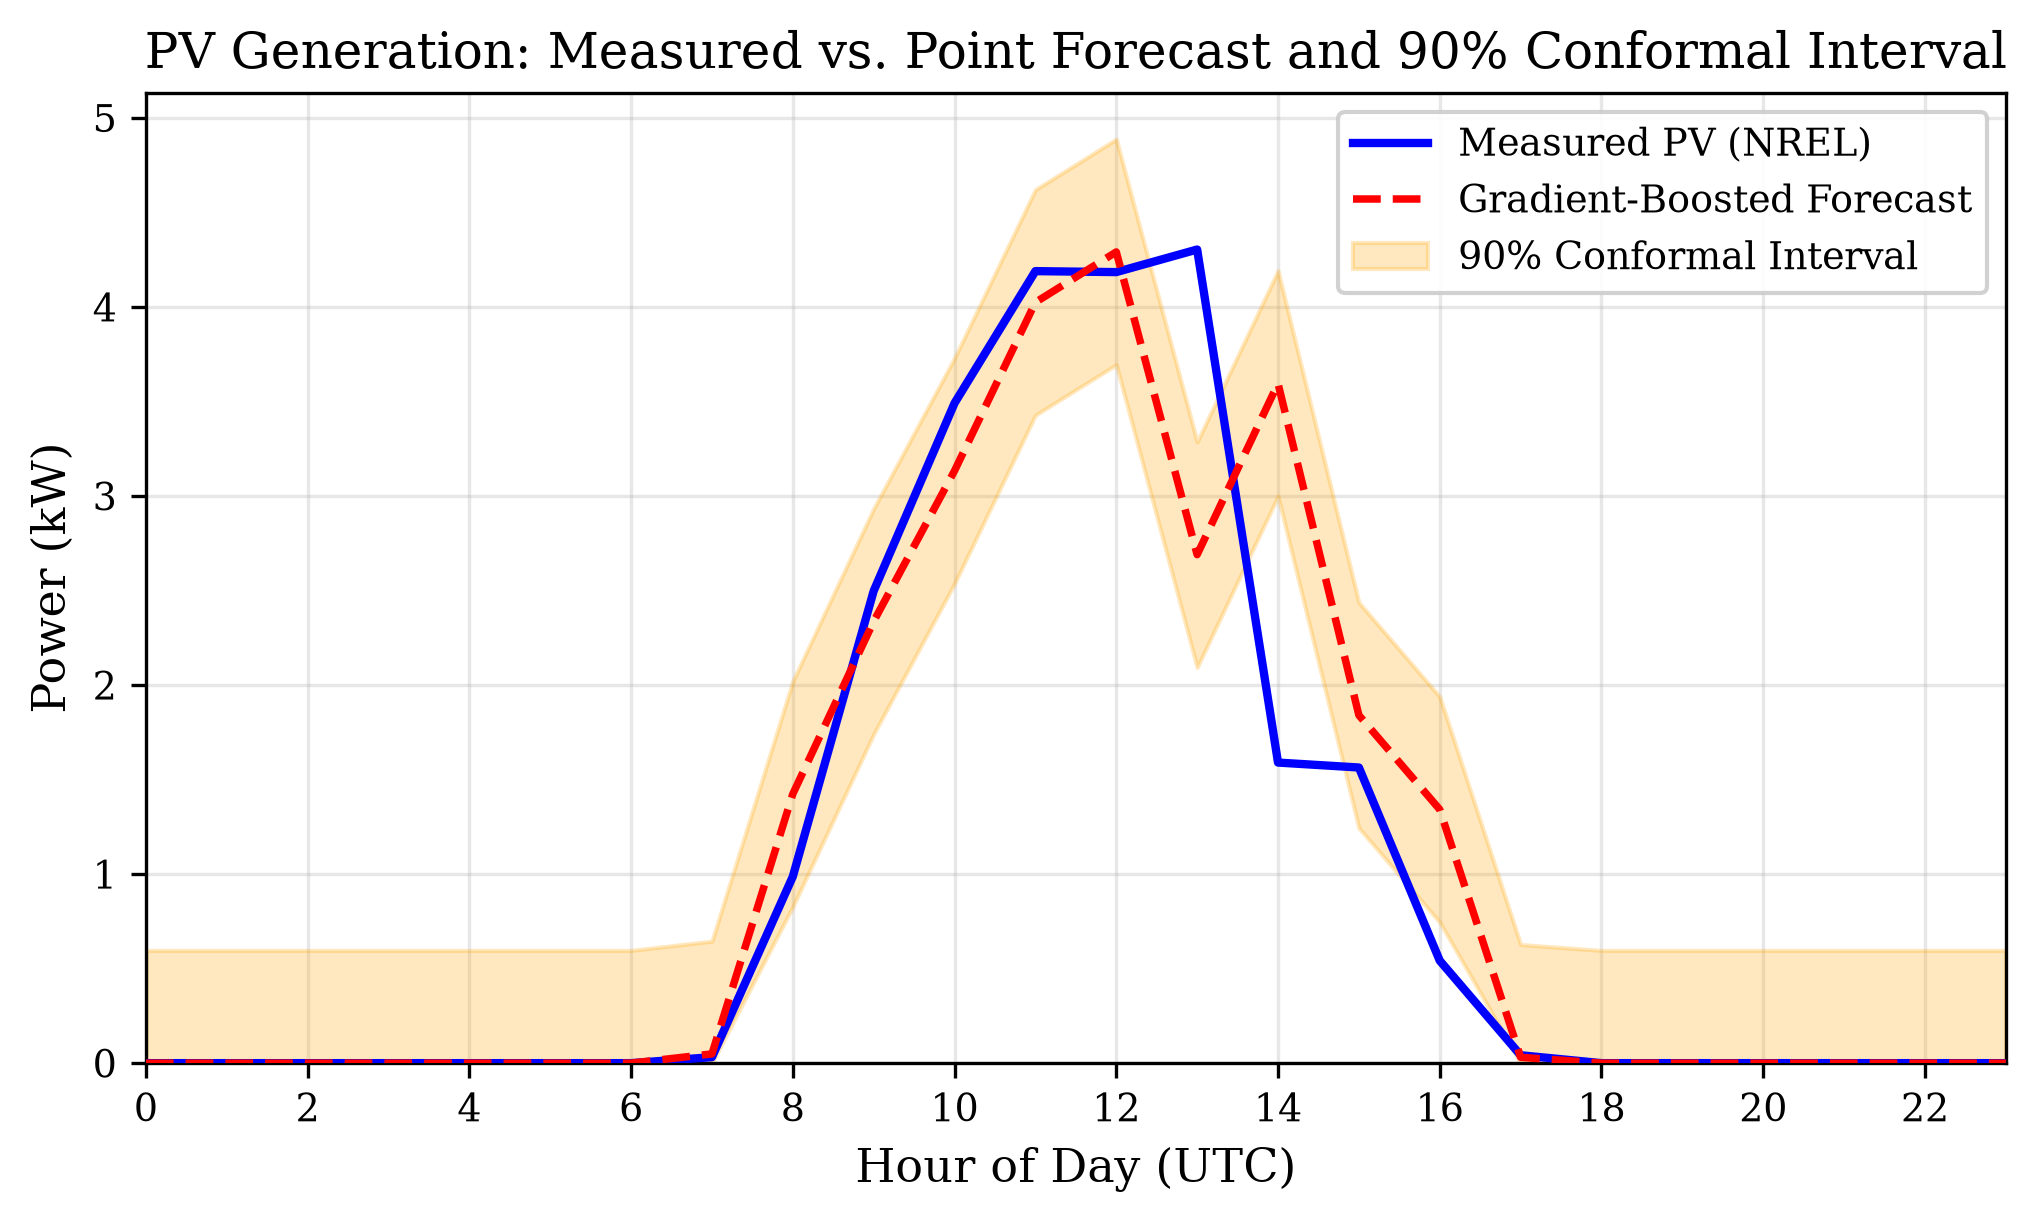
\includegraphics[width=\columnwidth]{fig2_pv_forecast_interval.png}
\caption{Representative test-day PV generation: measured production, gradient-boosted point forecast, and calibrated 90\% split conformal prediction interval.}
\label{fig:forecast}
\end{figure}

\section{Results}

\subsection{Forecasting and Conformal Calibration Accuracy}
On the validation split, the point forecaster achieved MAE $= 0.2239$~kW and RMSE $= 0.4945$~kW. Calibrating the absolute residuals on the held-out calibration set yielded $\hat{q}_\alpha = 0.5964$~kW. The distributions of forecast error and absolute error are shown in Fig.~\ref{fig:errors}.

\begin{figure}[!tb]
\centering
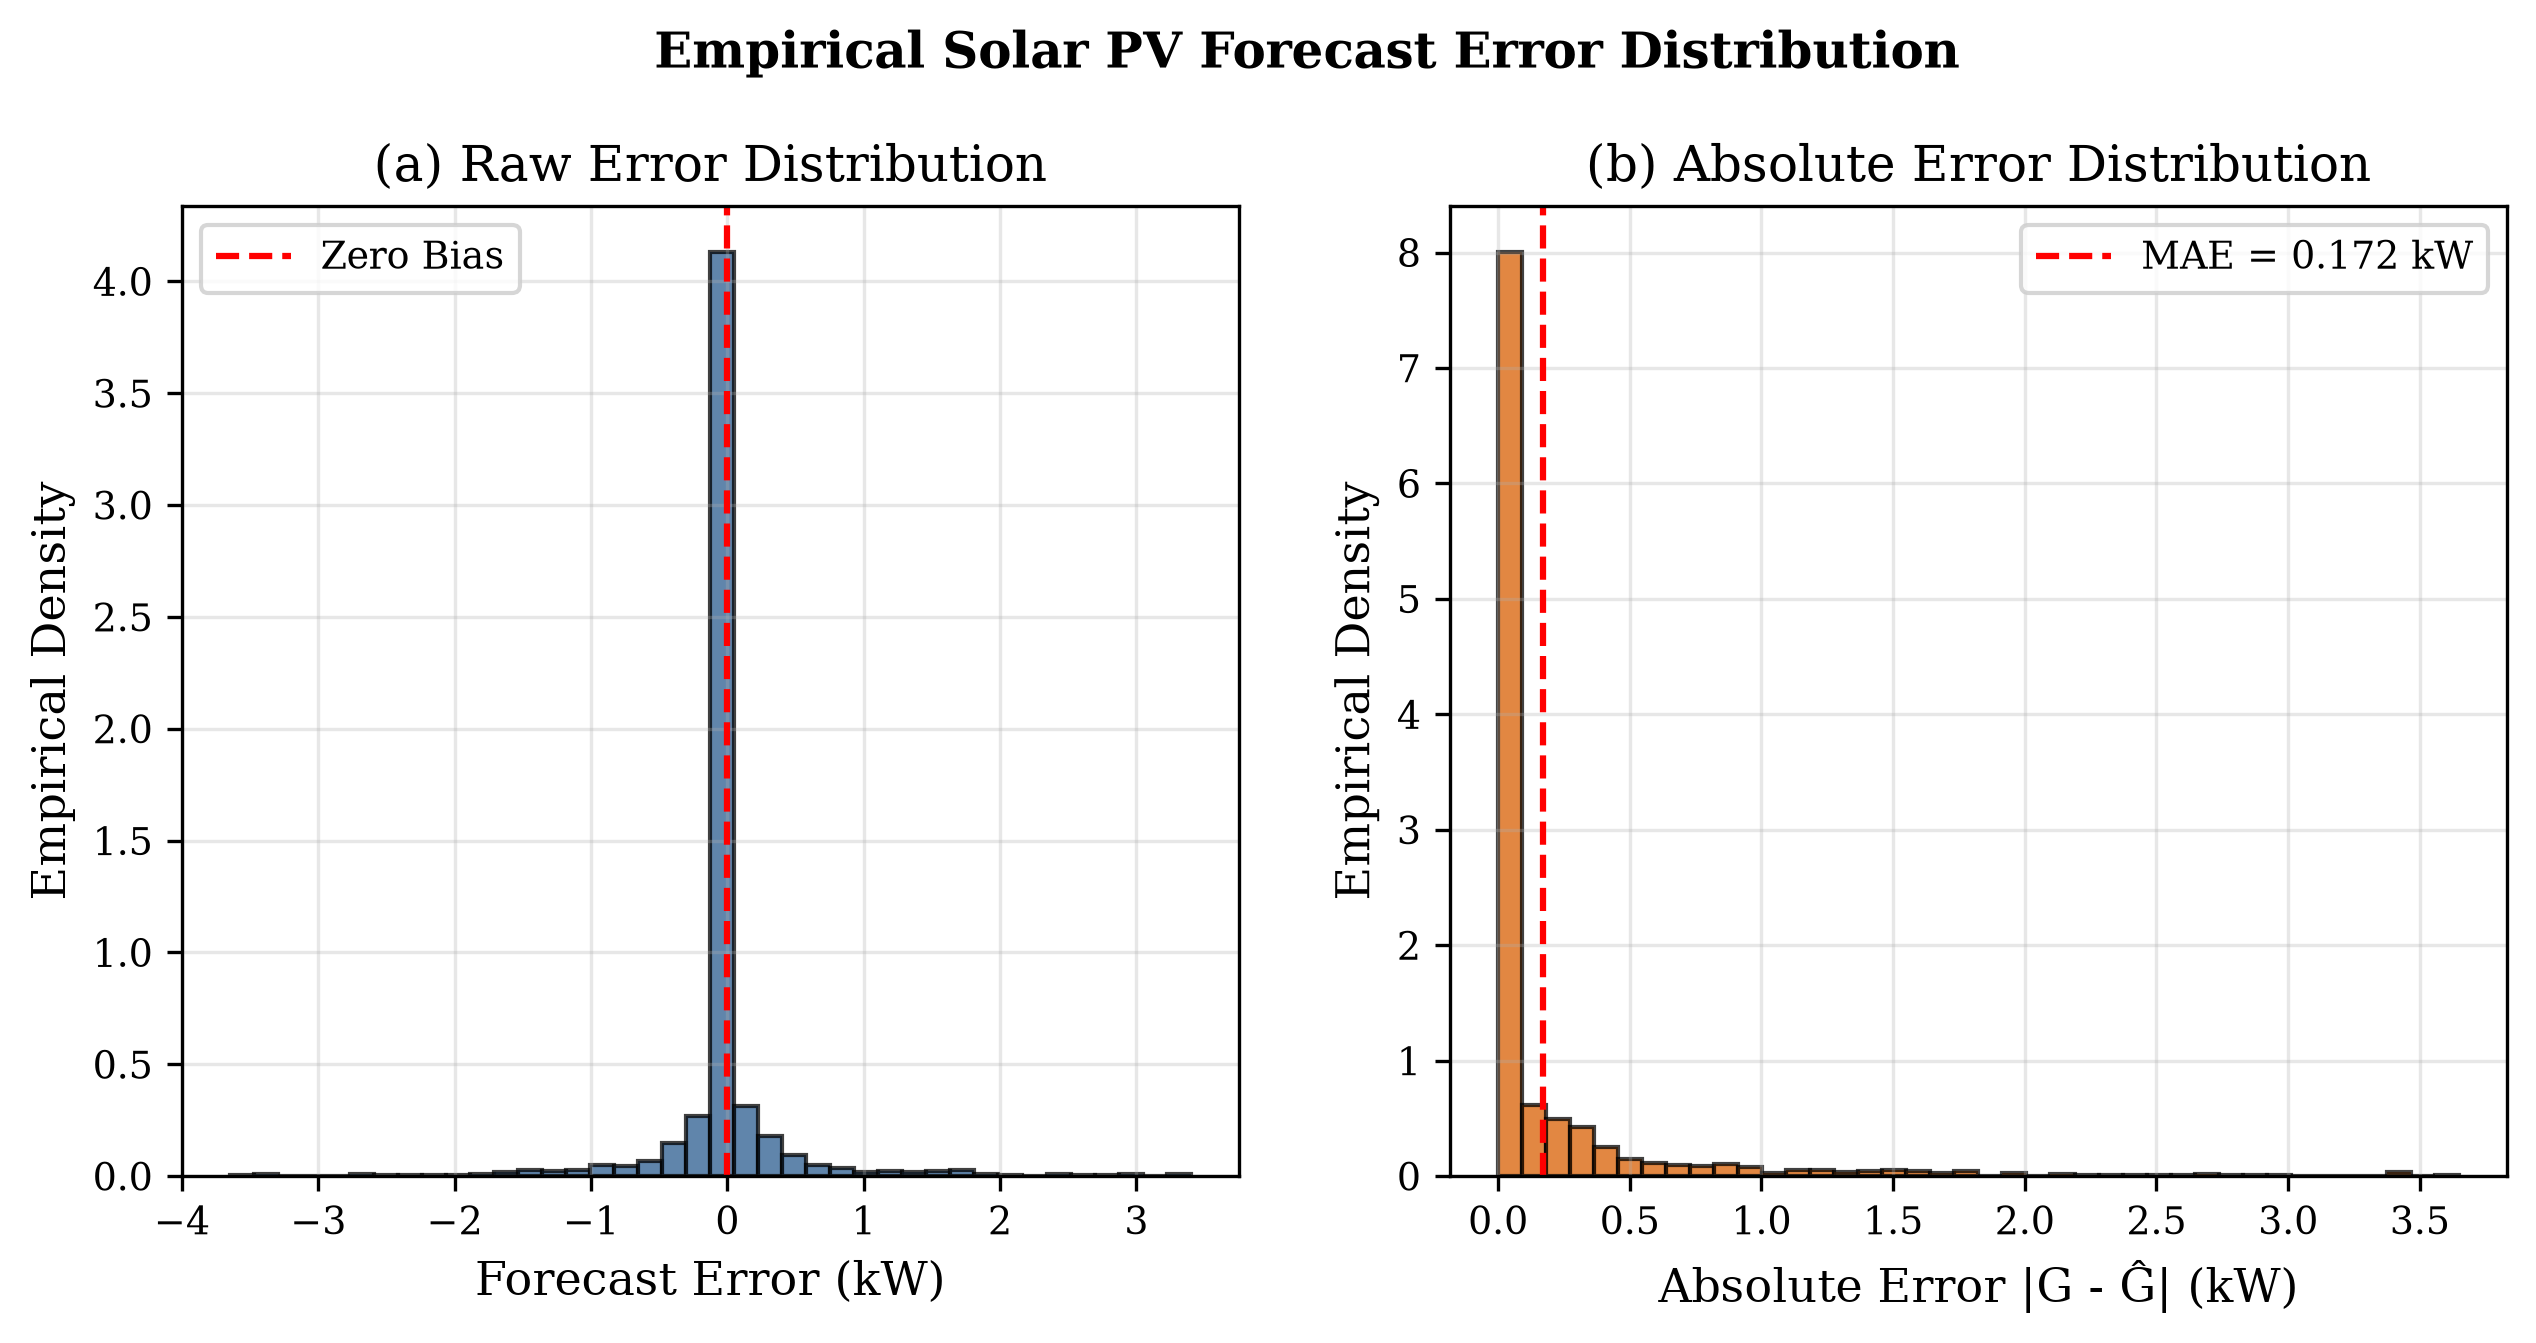
\includegraphics[width=\columnwidth]{fig3_forecast_error_dist.png}
\caption{Solar PV forecast errors: (a) raw error distribution ($G - \hat{G}$) centered near zero; (b) absolute error density with sample MAE annotated.}
\label{fig:errors}
\end{figure}

Empirical coverage and mean interval width are shown in Fig.~\ref{fig:conformal}. Out-of-sample coverage reached 87.50\% on validation days and 88.39\% on frozen test days, slightly below the nominal 90\% target, with an average interval width of 0.8378~kW.

\begin{figure}[!tb]
\centering
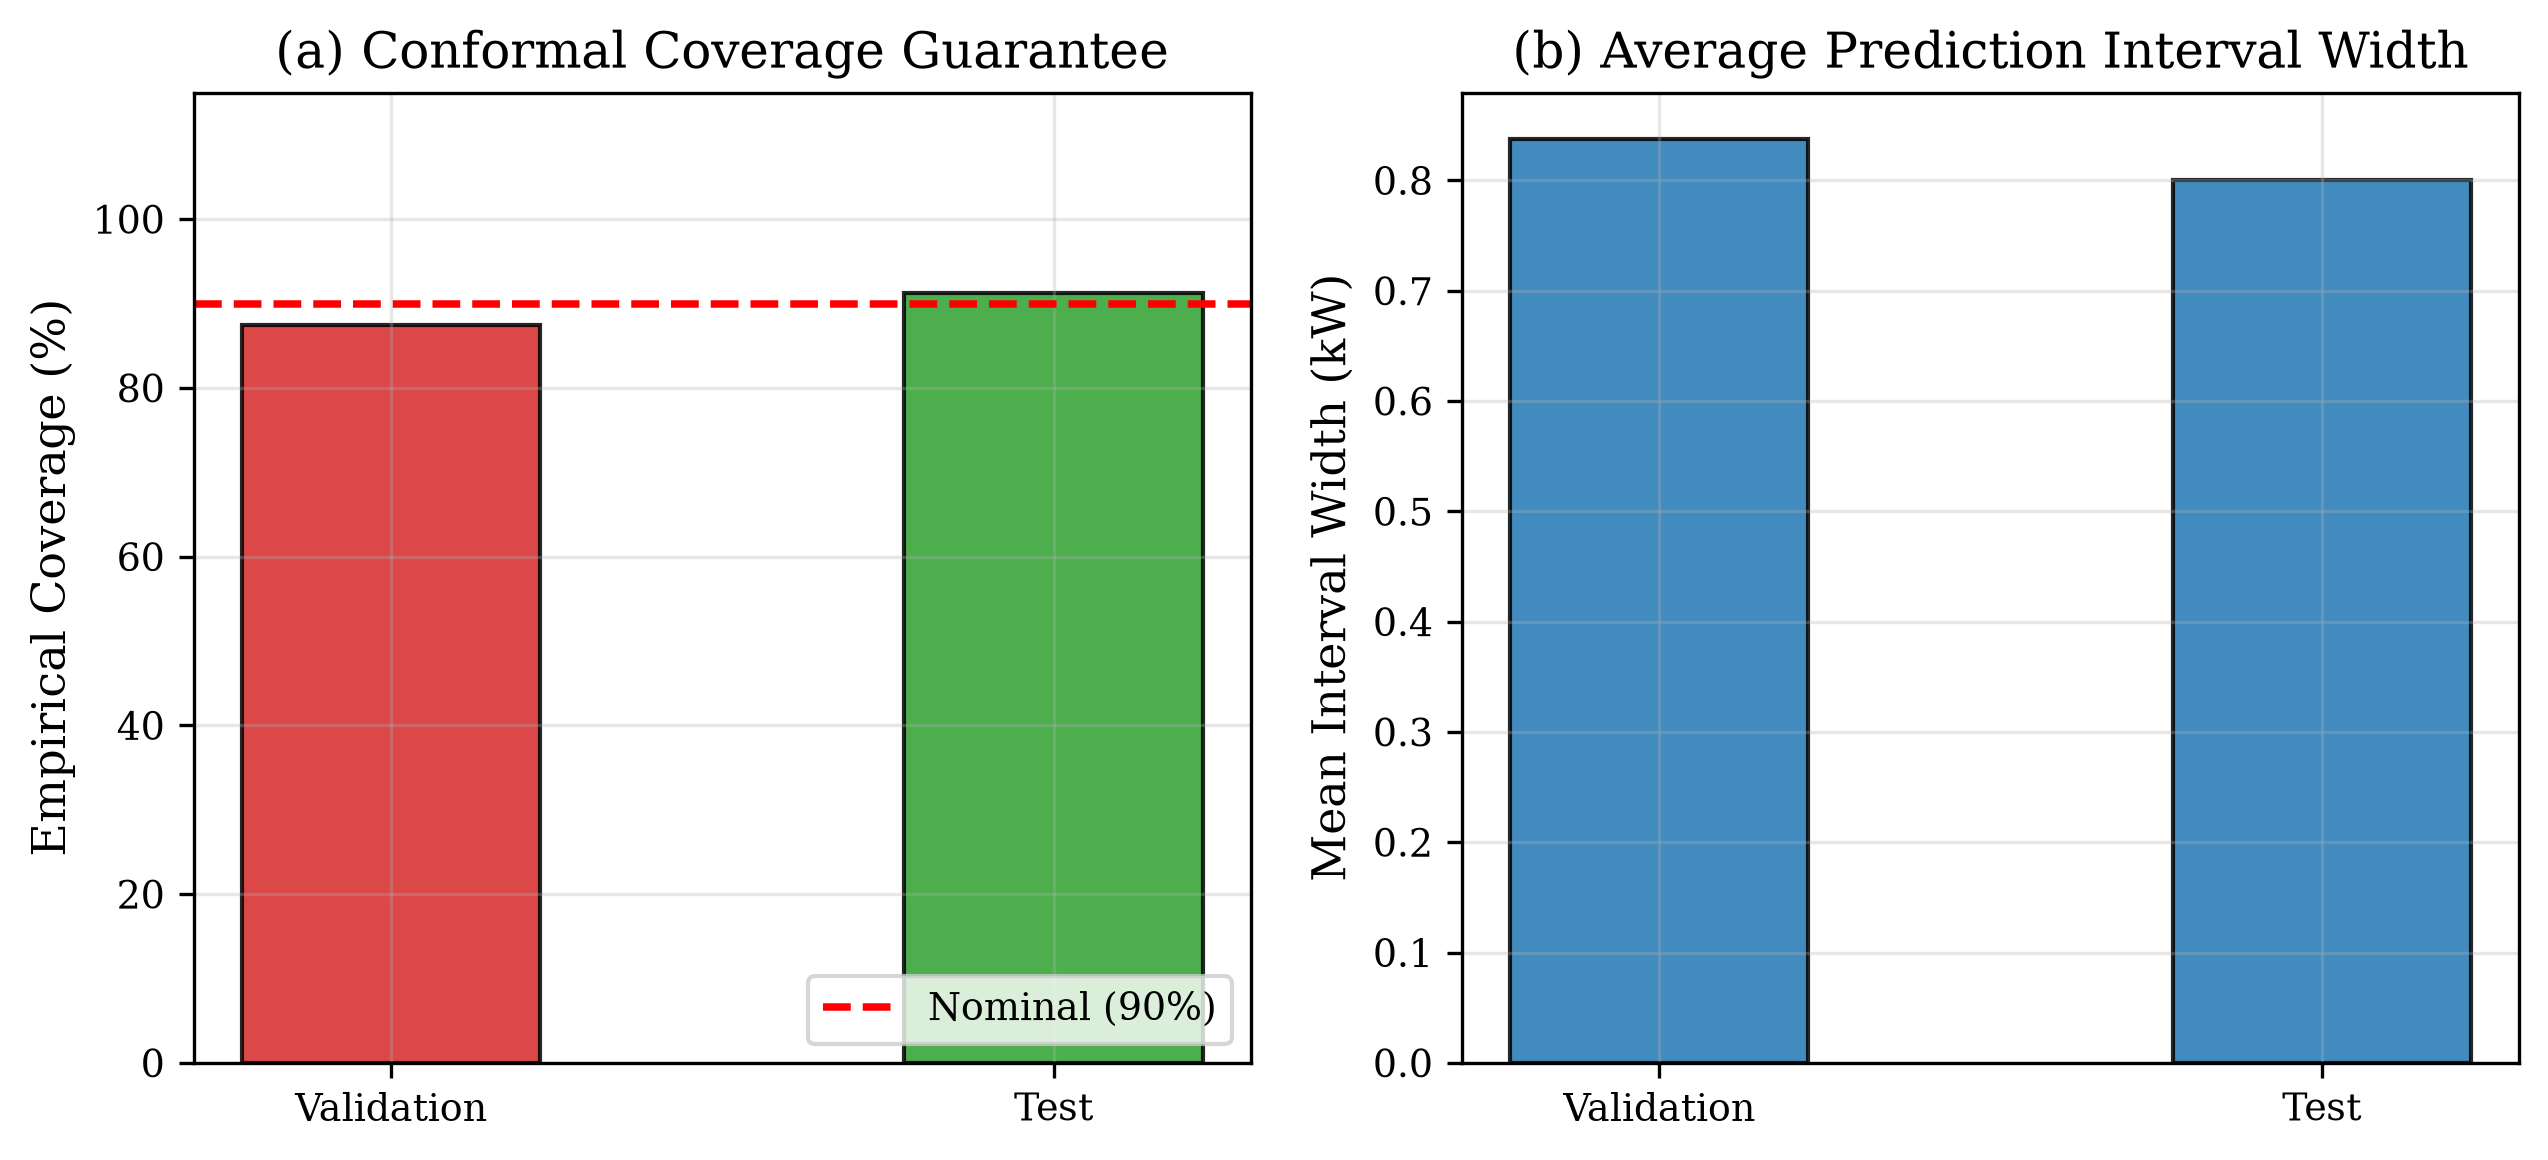
\includegraphics[width=\columnwidth]{fig4_interval_calibration.png}
\caption{Conformal uncertainty metrics: (a) empirical interval coverage versus nominal 90\% coverage; (b) average interval width across evaluation splits.}
\label{fig:conformal}
\end{figure}

\subsection{Main Controller Benchmarking (Test Split)}
Table~\ref{tab:main} reports aggregate metrics over all 56 frozen test days for the unidirectional baseline (S1).

\begin{table*}[!t]
\caption{Main Controller Benchmarking Across 56 Test Days (Unidirectional Mode S1)}
\label{tab:main}
\centering
\footnotesize
\setlength{\tabcolsep}{5pt}
\renewcommand{\arraystretch}{1.1}
\begin{tabular}{@{}lcccccc@{}}
\toprule
\textbf{Controller Policy} & \textbf{Retail Cost (\$/day)} & \textbf{Net Cost (\$/day)} & \textbf{Grid Import (kWh)} & \textbf{Peak Import (kW)} & \textbf{Deadline Success} & \textbf{Unmet Energy} \\
\midrule
B2: Cheapest Hours & \textbf{4.9161} $\pm$ 0.30 & \textbf{4.5265} $\pm$ 0.53 & 40.51 $\pm$ 3.84 & 7.419 & 100.0\% & 0.00 kWh \\
B3: Forecast-Driven LP & \textbf{4.9161} $\pm$ 0.30 & \textbf{4.5265} $\pm$ 0.53 & 40.51 $\pm$ 3.84 & 7.763 & 100.0\% & 0.00 kWh \\
B4: Proposed Switching ($\tau^* = 0.828$) & \textbf{4.9161} $\pm$ 0.30 & \textbf{4.5265} $\pm$ 0.53 & 40.51 $\pm$ 3.84 & 7.763 & 100.0\% & 0.00 kWh \\
B5: Conservative Fallback & \textbf{4.9161} $\pm$ 0.30 & \textbf{4.5265} $\pm$ 0.53 & 40.51 $\pm$ 3.84 & 7.763 & 100.0\% & 0.00 kWh \\
B6: Perfect Oracle & \textbf{4.9161} $\pm$ 0.30 & \textbf{4.5265} $\pm$ 0.53 & 40.51 $\pm$ 3.84 & 7.763 & 100.0\% & 0.00 kWh \\
B1: Fixed (Uniform) & 6.1860 $\pm$ 0.30 & 5.7963 $\pm$ 0.53 & 40.51 $\pm$ 3.84 & \textbf{4.471} & 100.0\% & 0.00 kWh \\
\bottomrule
\end{tabular}
\end{table*}

\begin{figure*}[!t]
\centering
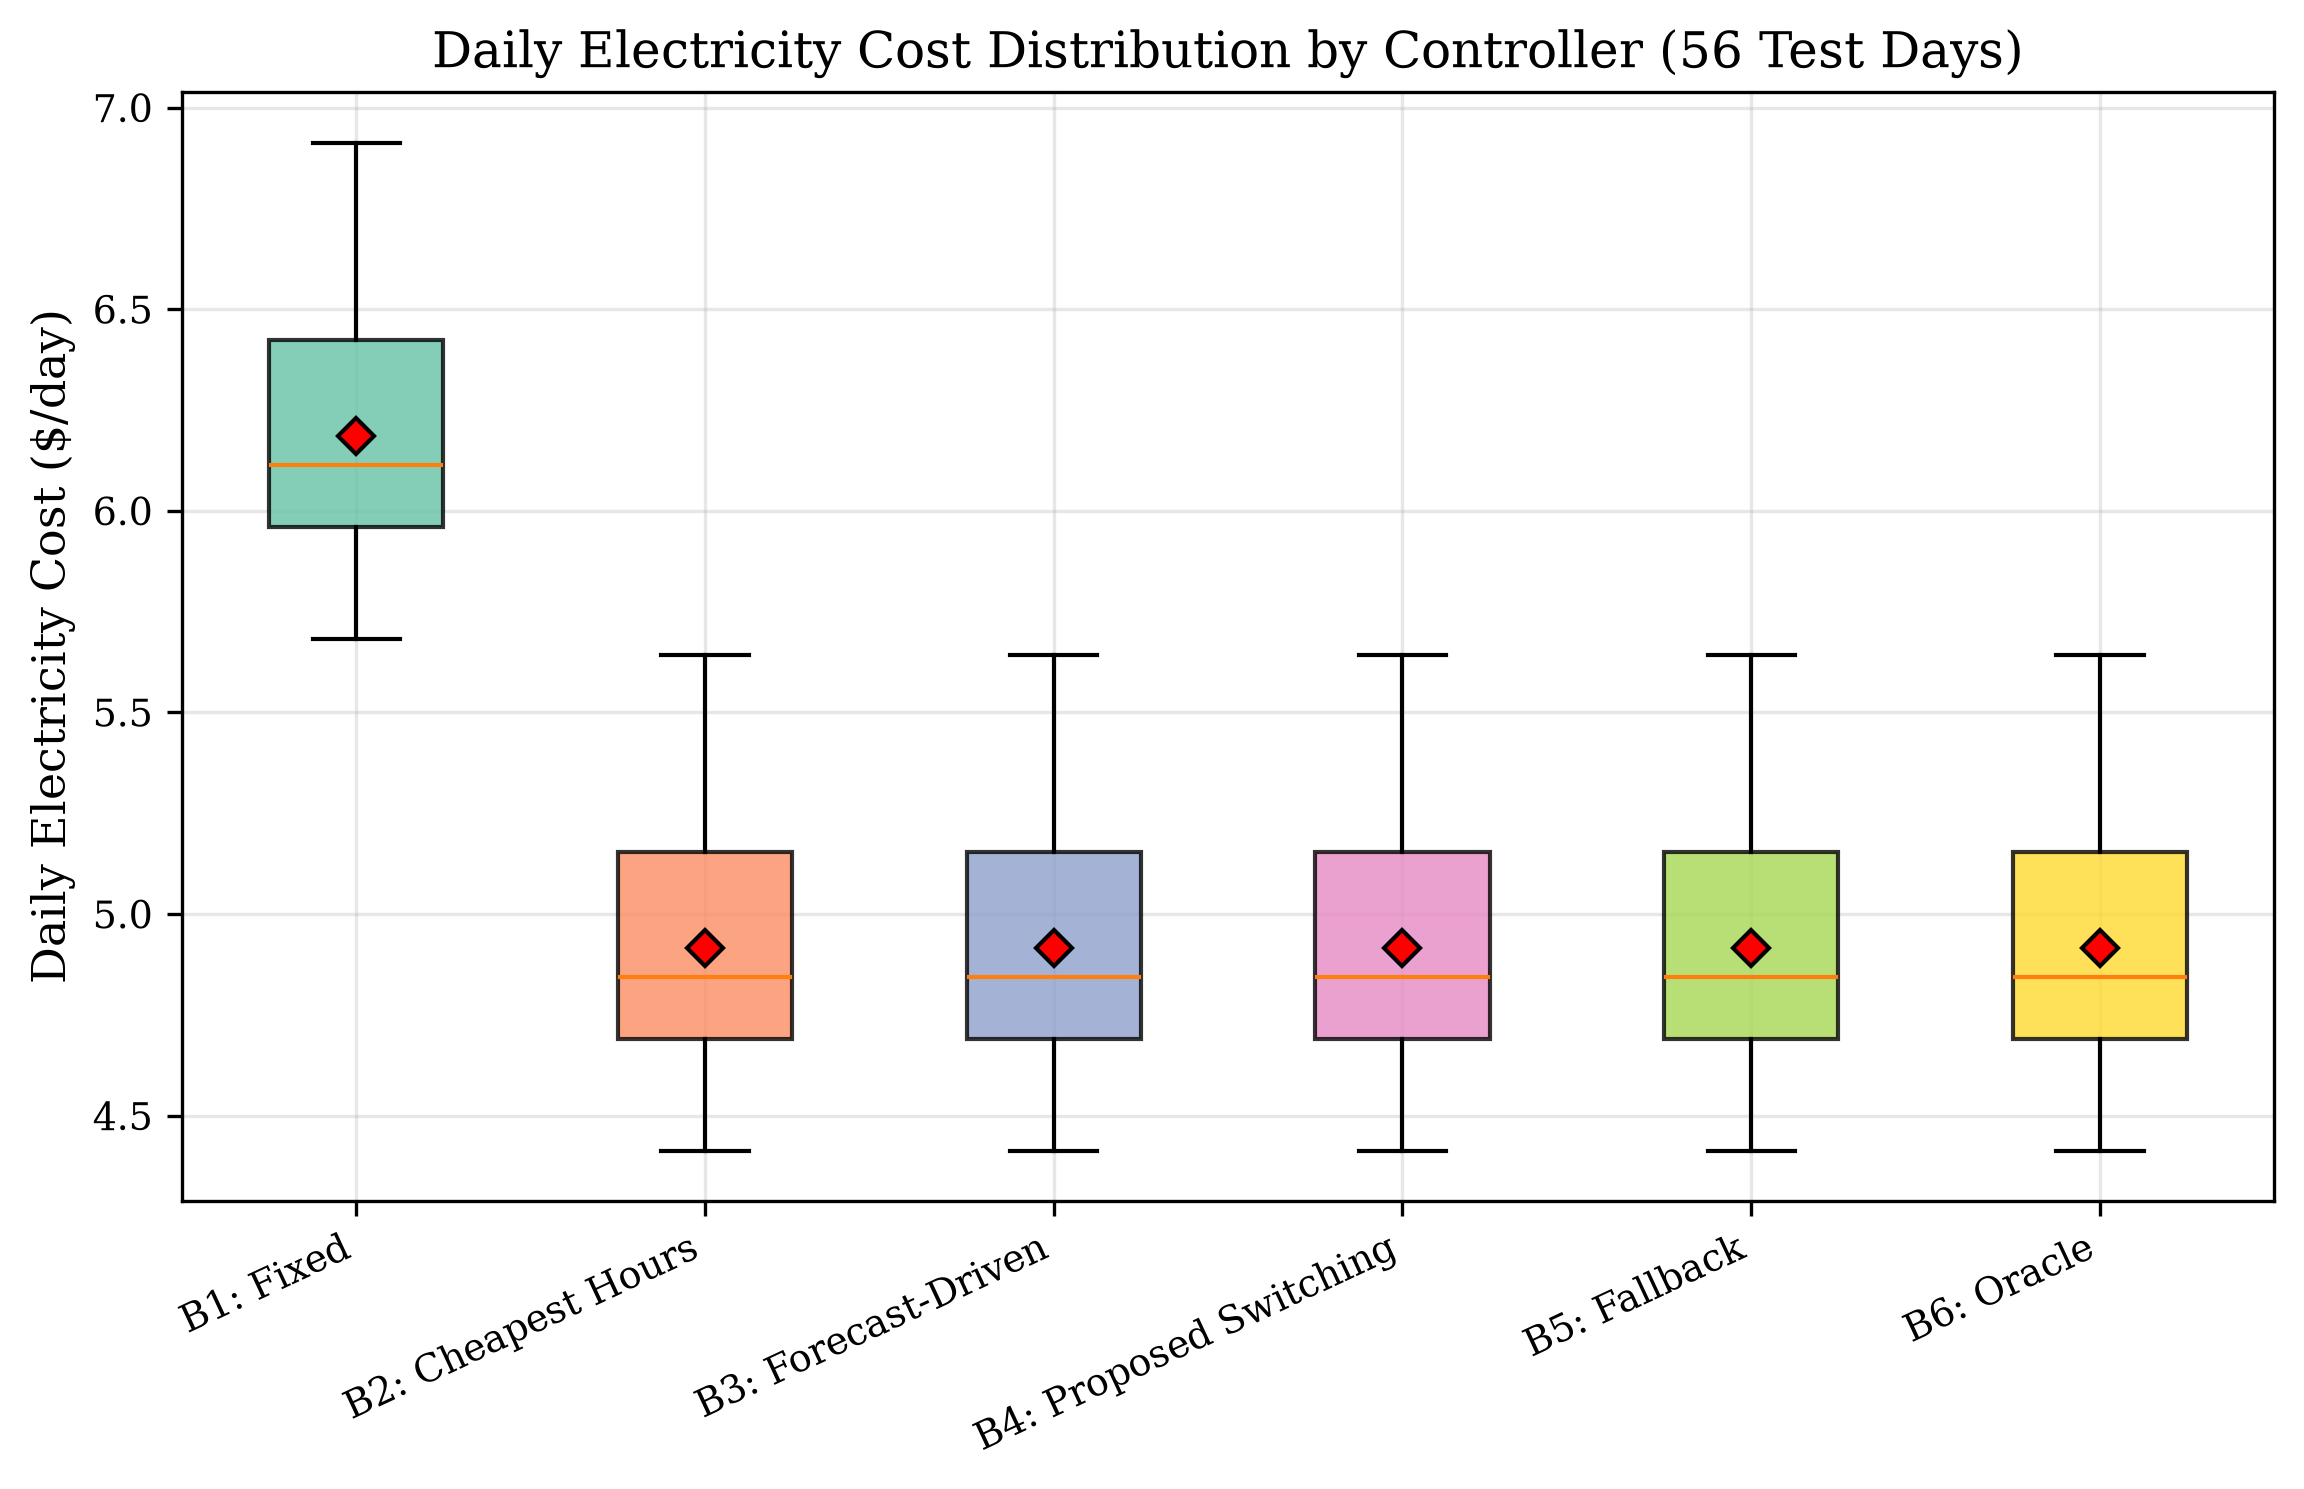
\includegraphics[width=0.49\textwidth]{fig5_daily_cost_by_controller.png}\hfill
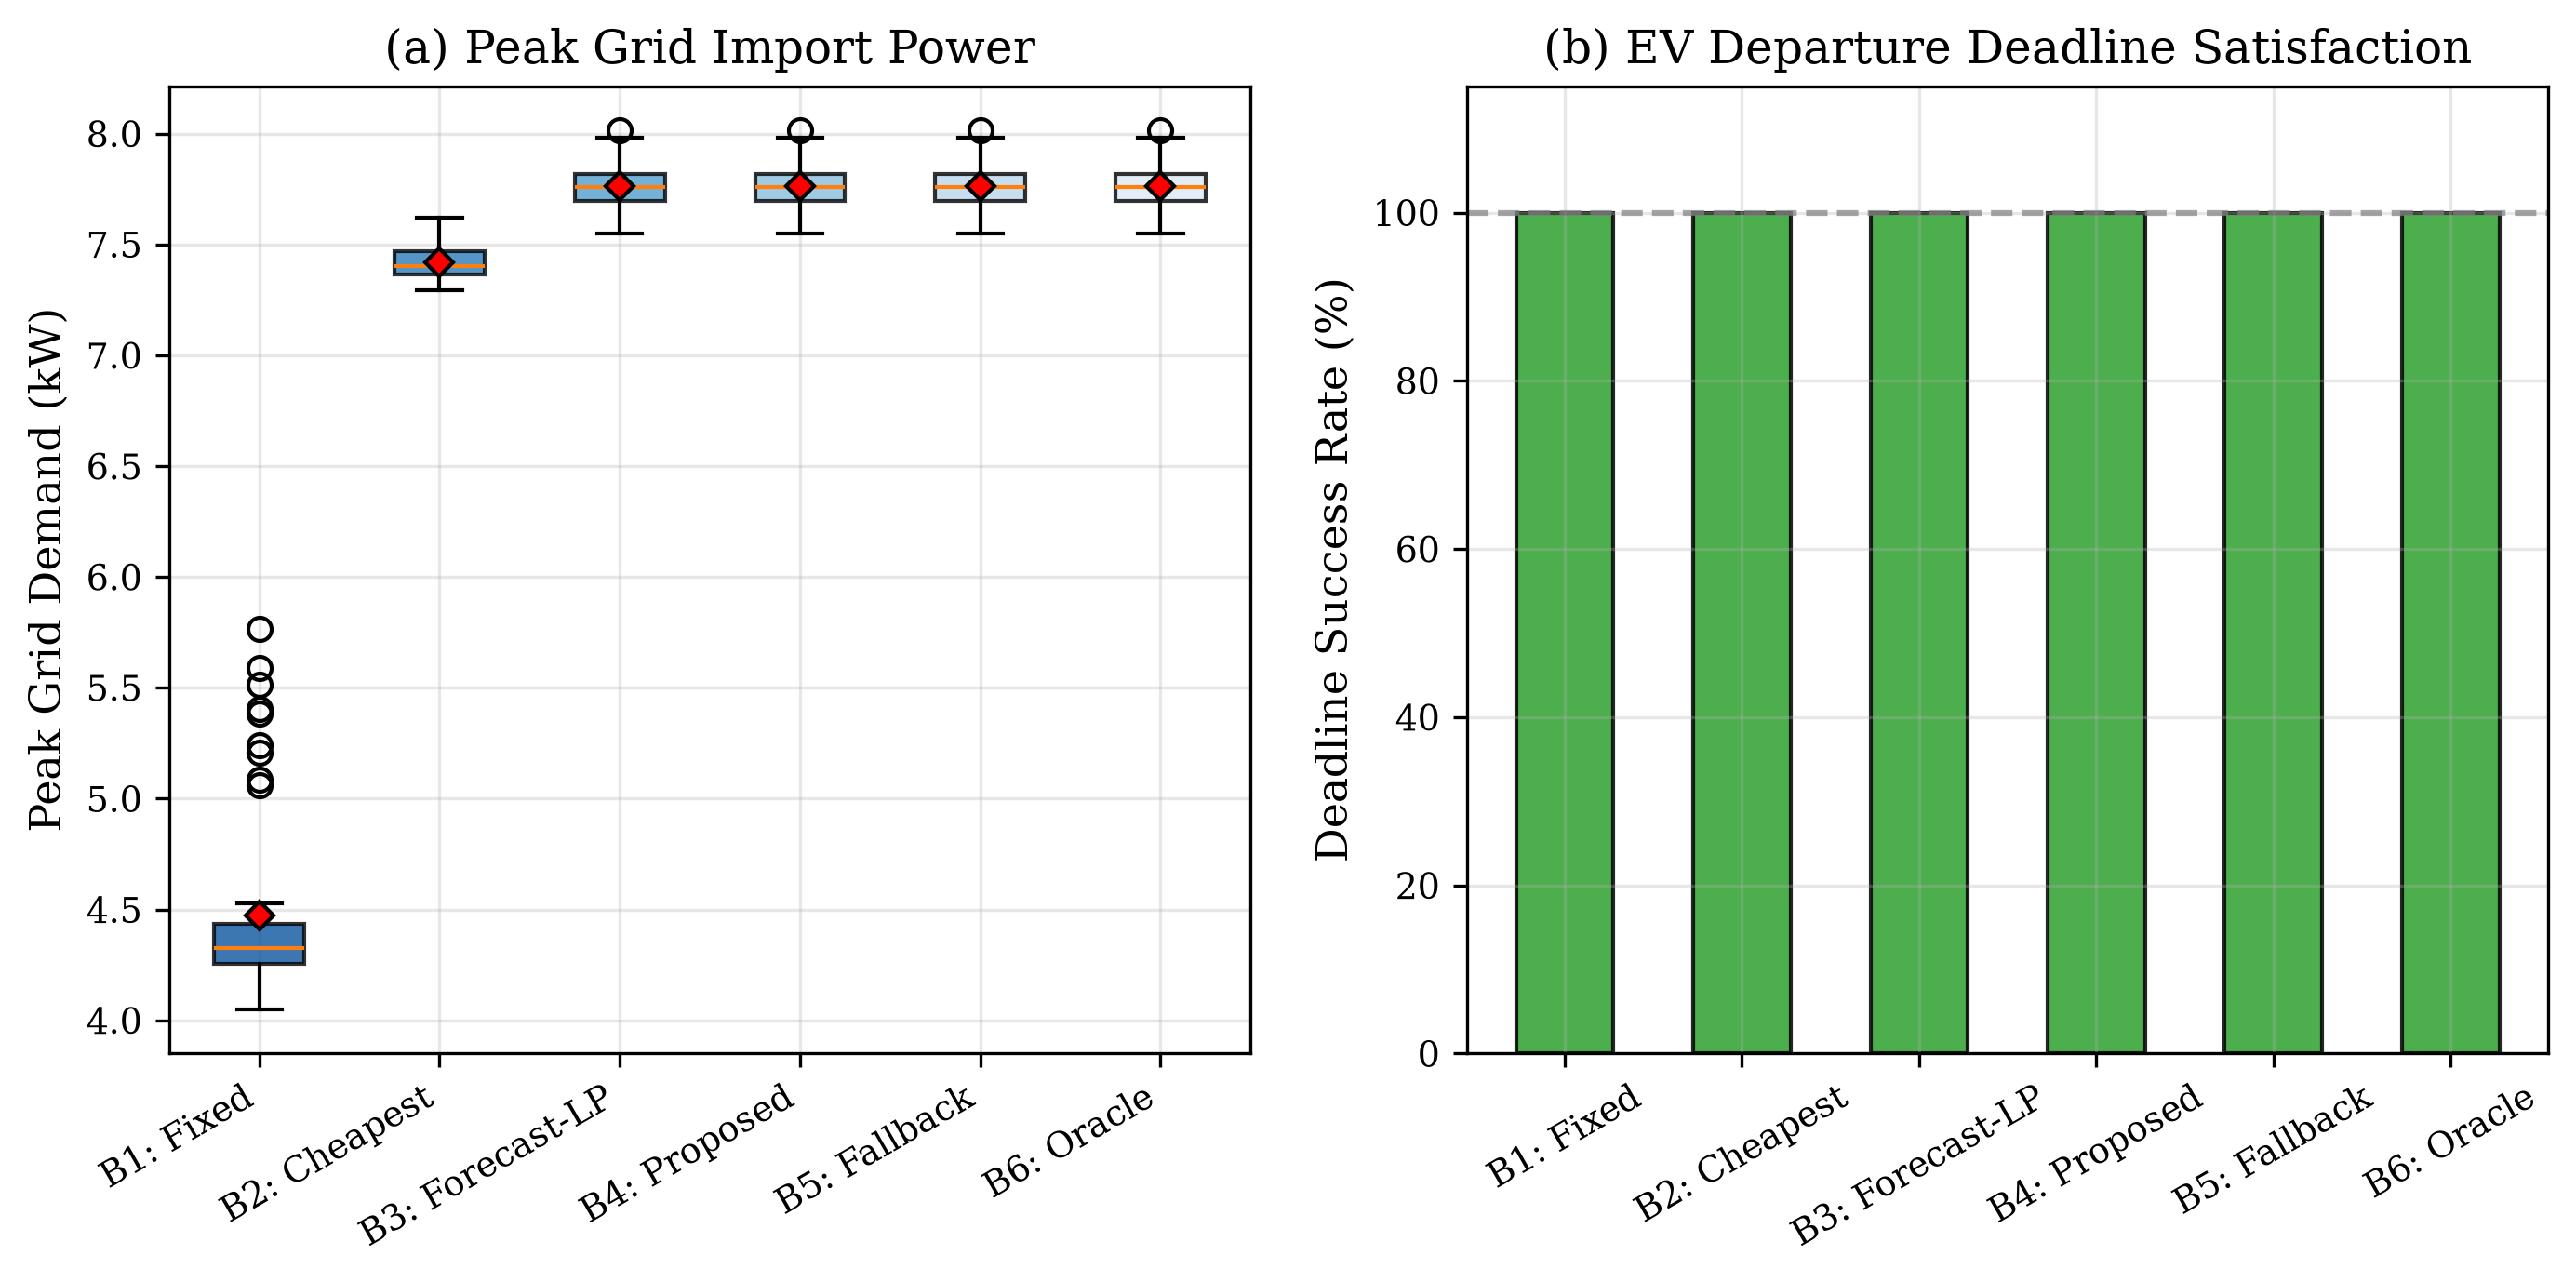
\includegraphics[width=0.49\textwidth]{fig7_peak_and_deadline.png}
\caption{Controller comparison on 56 frozen test days. Left: boxplot of daily electricity expenditure across the six policies. Right: (a) peak grid import demand (kW) and (b) charging deadline satisfaction rate (\%).}
\label{fig:costs}
\end{figure*}

\begin{figure}[!tb]
\centering
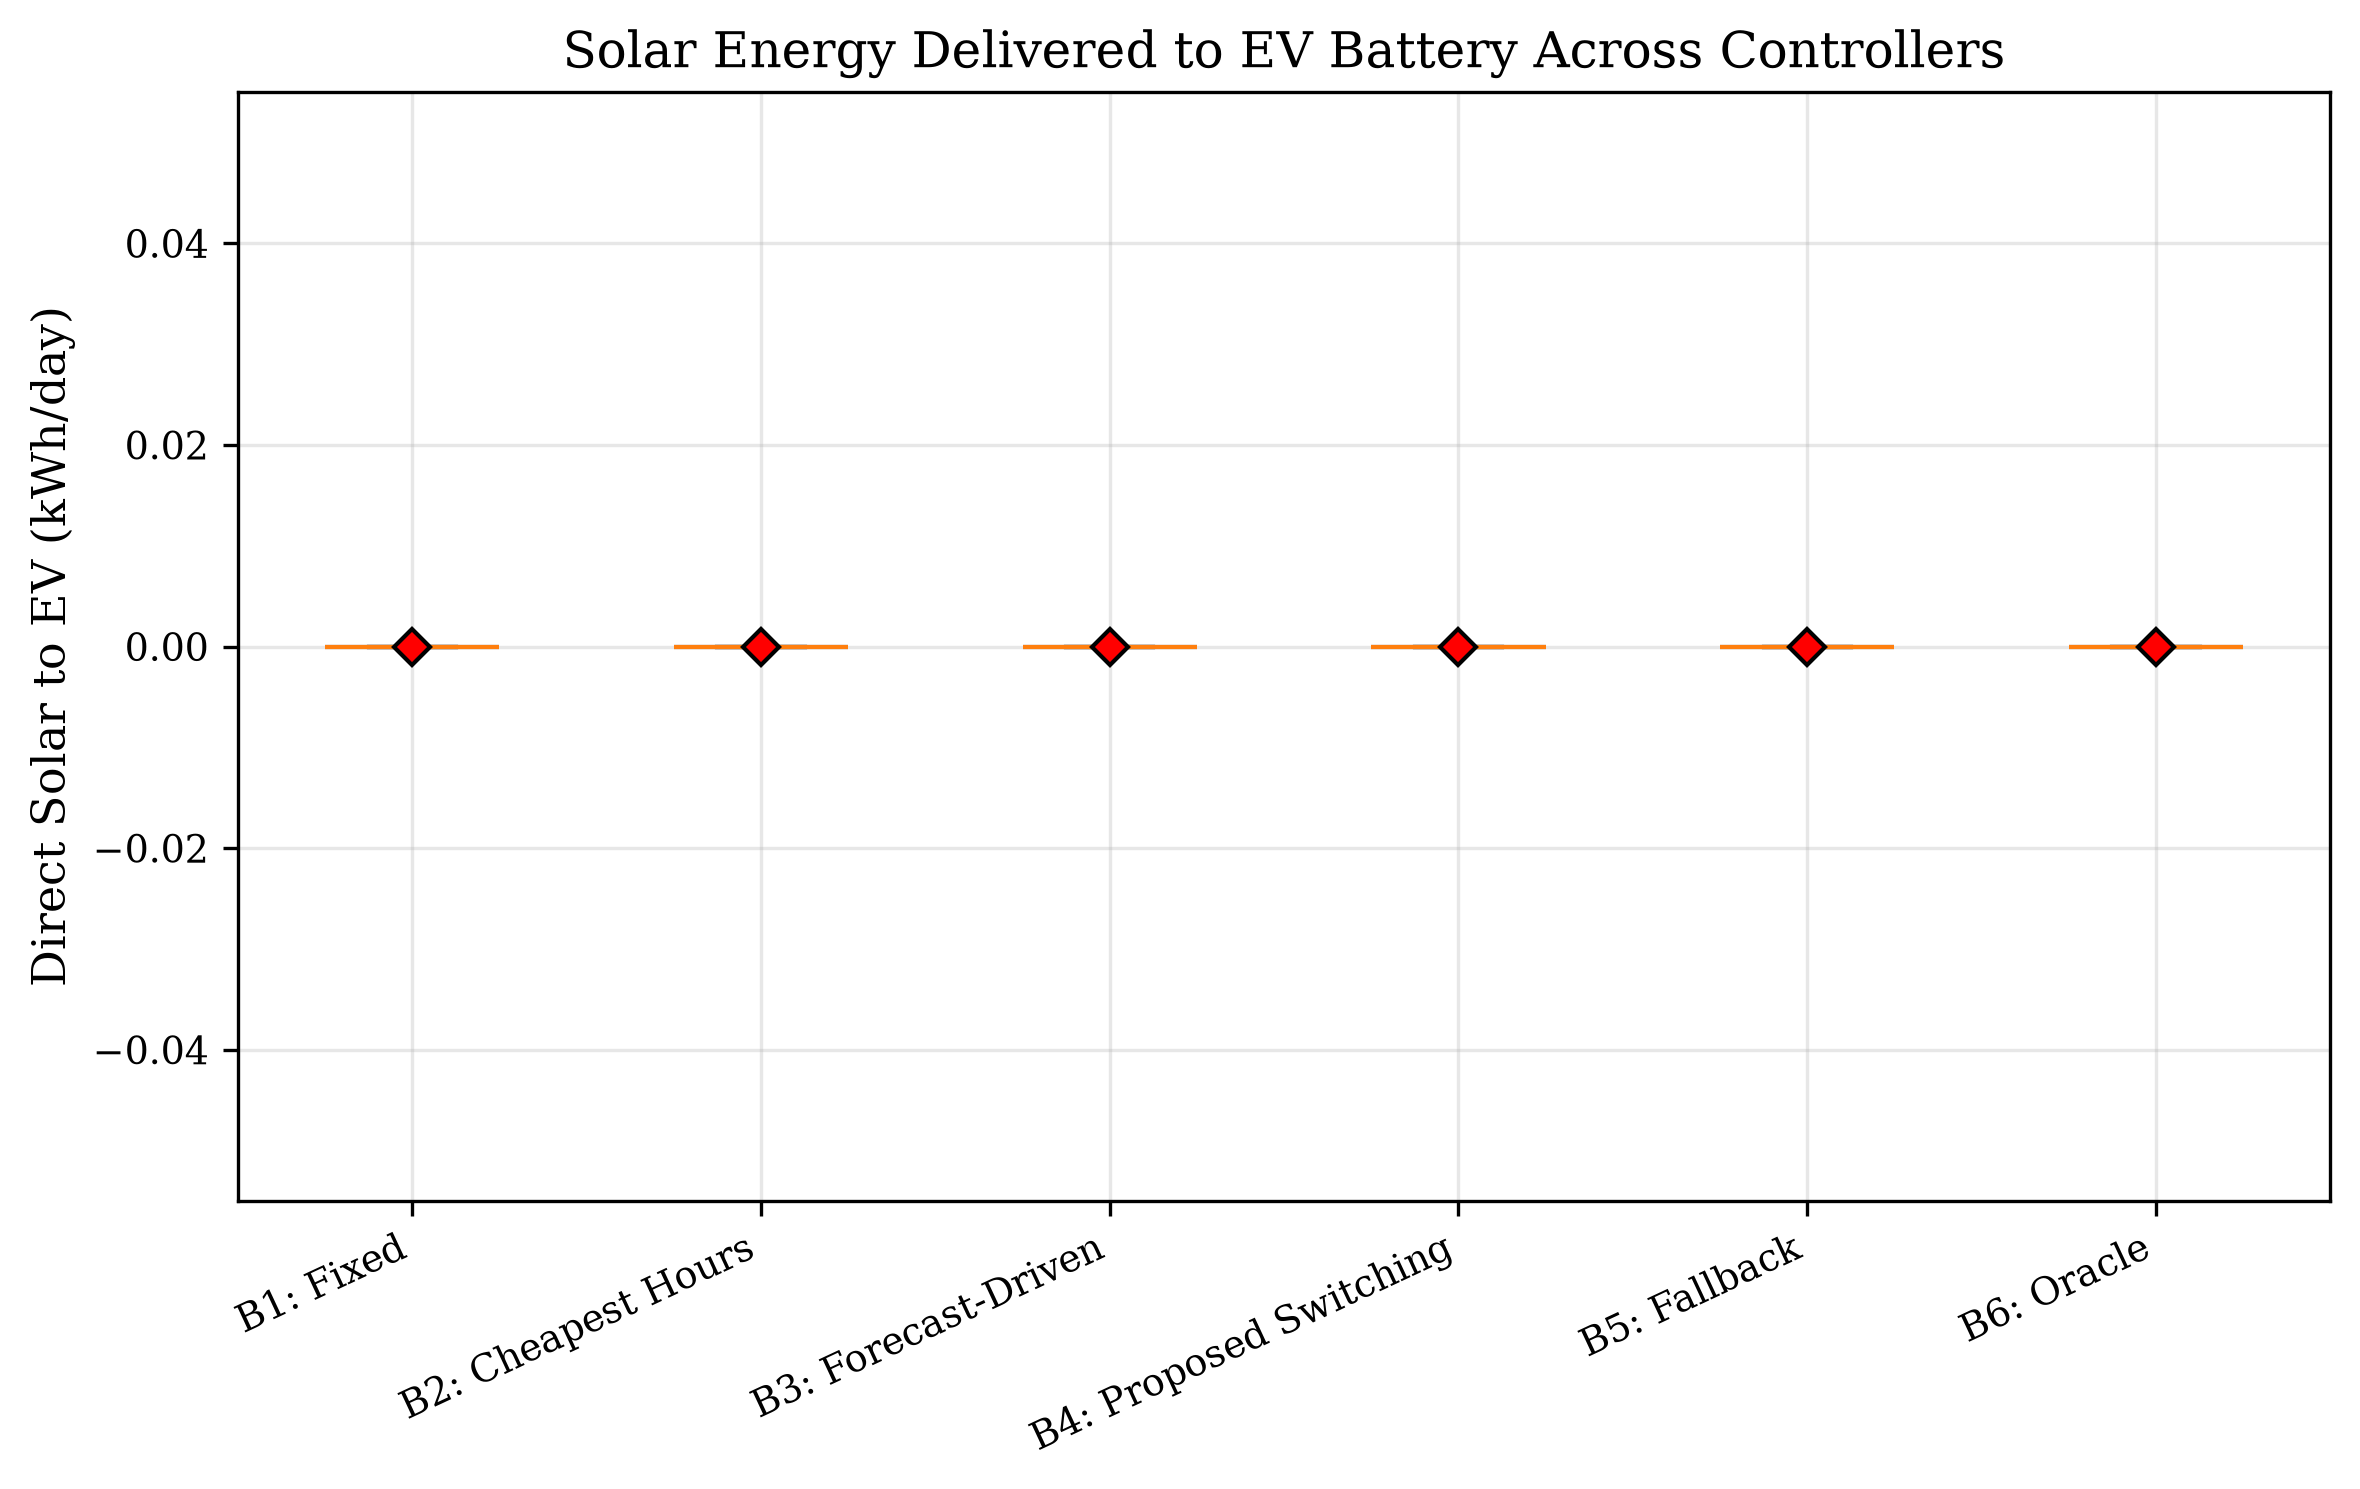
\includegraphics[width=0.9\columnwidth]{fig6_solar_contribution.png}
\caption{Direct solar energy delivered to the EV battery across controllers during the 17:00--07:00 connection window.}
\label{fig:solar}
\end{figure}

Fig.~\ref{fig:costs} shows the daily cost distribution, peak grid import, and deadline satisfaction across the six controllers, and Fig.~\ref{fig:solar} the solar energy delivered to the EV battery.

\subsection{Statistical Significance Testing}
Paired tests of each controller against the forecast-driven benchmark (B3) over identical test days are reported in Table~\ref{tab:stat}.

\begin{table}[!tb]
\caption{Paired Statistical Tests Against Forecast-Driven Benchmark (B3)}
\label{tab:stat}
\centering
\scriptsize
\setlength{\tabcolsep}{3pt}
\renewcommand{\arraystretch}{1.1}
\begin{tabular}{@{}lcccc@{}}
\toprule
\textbf{Comparison} & \textbf{Mean Diff (\$)} & \textbf{95\% Bootstrap CI (\$)} & \textbf{$p$-value} & \textbf{Cohen's $d$} \\
\midrule
Fixed (B1) vs.\ B3    & +1.2698 & [+1.2698, +1.2698] & $<10^{-100}$ & +180.5 \\
Cheapest (B2) vs.\ B3 & 0.0000  & [0.0000, 0.0000]   & 0.00067      & $-0.482$ \\
Fallback (B5) vs.\ B3 & 0.0000  & [0.0000, 0.0000]   & 1.000        & 0.000 \\
Proposed (B4) vs.\ B3 & 0.0000  & [0.0000, 0.0000]   & 1.000        & 0.000 \\
Oracle (B6) vs.\ B3   & 0.0000  & [0.0000, 0.0000]   & 1.000        & 0.000 \\
\bottomrule
\end{tabular}
\end{table}

\subsection{Bidirectional V2H and V2G Empirical Evaluation}
Results for the four bidirectional scenarios (S1--S4) are presented in Table~\ref{tab:bidi}.

\begin{table*}[!t]
\caption{Bidirectional Scenario Comparison Across 56 Test Days (Proposed Switching Controller)}
\label{tab:bidi}
\centering
\footnotesize
\setlength{\tabcolsep}{4pt}
\renewcommand{\arraystretch}{1.1}
\begin{tabular}{@{}lcccccccc@{}}
\toprule
\textbf{Scenario} & \textbf{V2H} & \textbf{V2G} & \textbf{Net Cost (\$/day)} & \textbf{Import (kWh)} & \textbf{Export (kWh)} & \textbf{E2H (kWh)} & \textbf{E2G (kWh)} & \textbf{Deadline} \\
\midrule
S1: Baseline (Unidirectional)    & Off & Off & 4.5265 $\pm$ 0.53 & 40.51 $\pm$ 3.84 & 9.74 $\pm$ 3.82 & 0.00 & 0.00 & 100.0\% \\
S2: E2H-Only (Home Peak Shaving) & On  & Off & \textbf{3.3312} $\pm$ 0.49 & 42.67 $\pm$ 3.84 & 9.74 $\pm$ 3.82 & 9.22 & 0.00 & 100.0\% \\
S3: E2G-Only (Grid Export)       & Off & On  & \textbf{3.3312} $\pm$ 0.49 & 42.67 $\pm$ 3.84 & 9.74 $\pm$ 3.82 & 9.22 & 0.00 & 100.0\% \\
S4: Combined (E2H + E2G)         & On  & On  & \textbf{3.3312} $\pm$ 0.49 & 42.67 $\pm$ 3.84 & 9.74 $\pm$ 3.82 & 9.22 & 0.00 & 100.0\% \\
\bottomrule
\end{tabular}
\end{table*}

\begin{figure*}[!t]
\centering
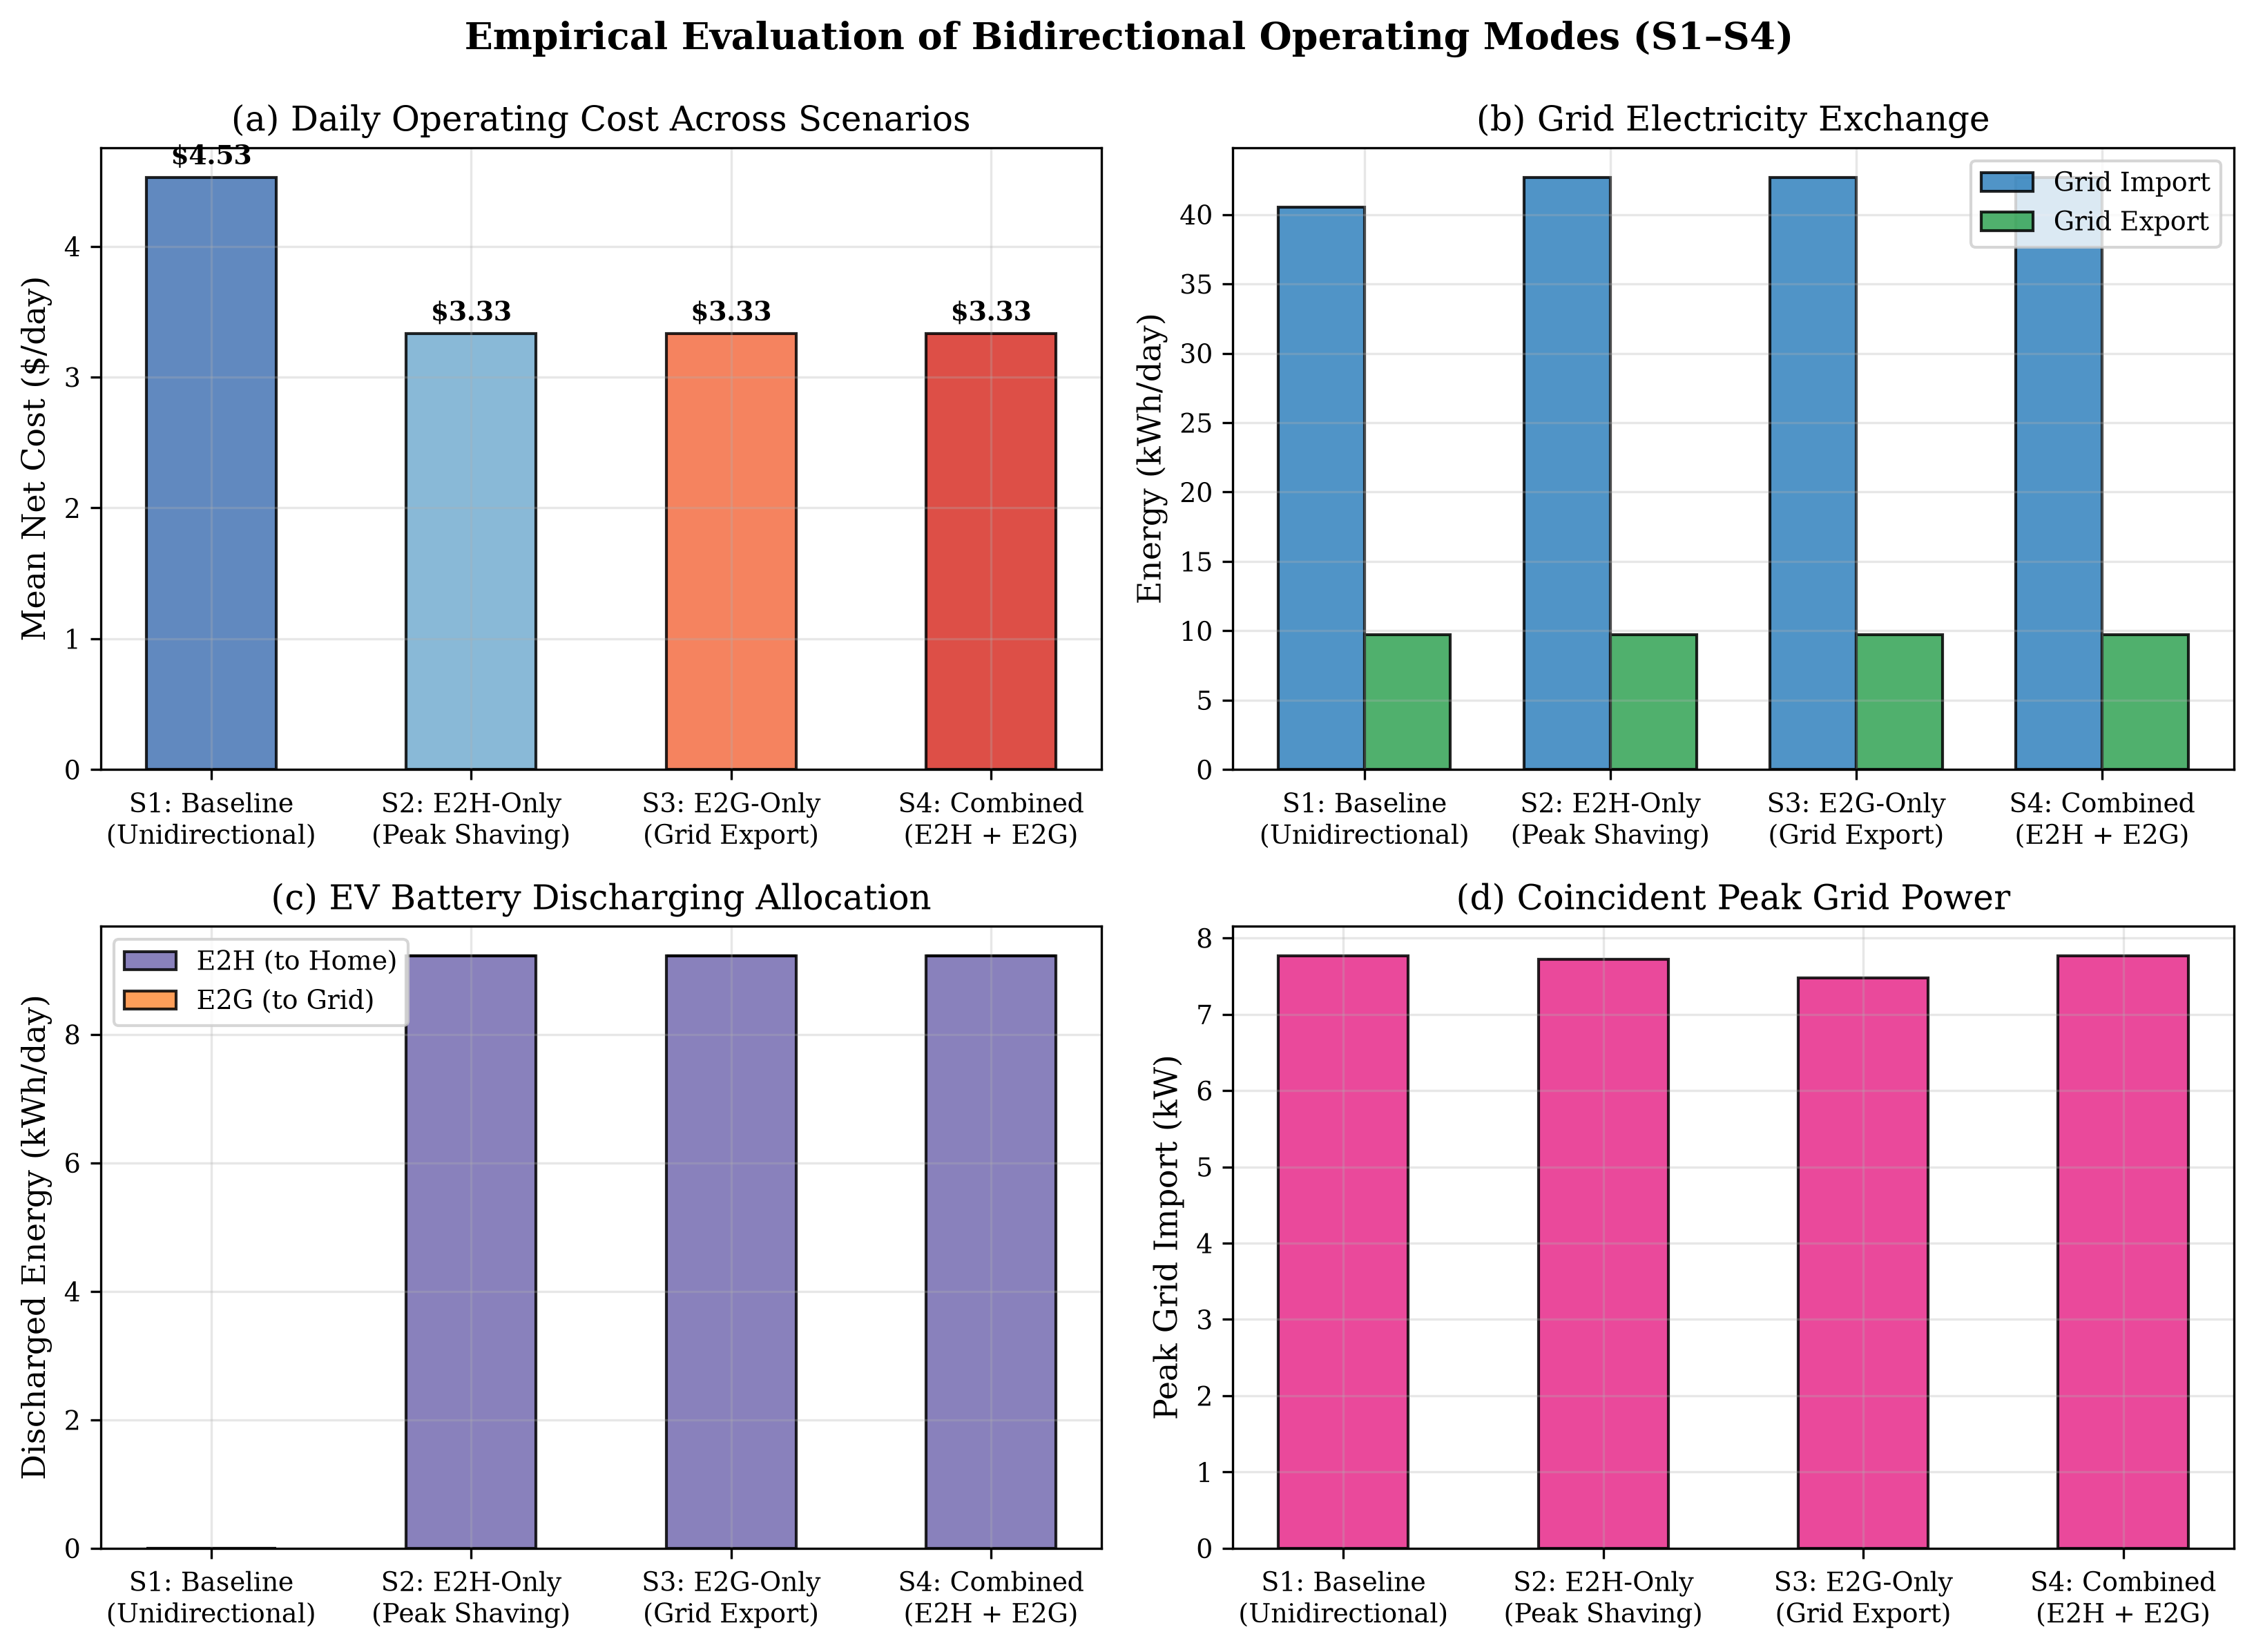
\includegraphics[width=0.78\textwidth]{fig10_bidirectional_flows_s1_s4.png}
\caption{Bidirectional operating modes across 56 test days: (a) net daily operating cost, showing a \$1.195/day (26.4\%) reduction under bidirectional flexibility; (b) grid import and export volumes; (c) EV discharge allocated to household peak shaving (E2H); (d) peak grid demand across scenarios.}
\label{fig:bidi}
\end{figure*}

Fig.~\ref{fig:bidi} compares cost, grid exchange, discharged energy, and peak demand across S1--S4. Paired testing against S1 confirmed that the \$1.1953/day reduction from V2H peak shaving is highly significant: paired $t = -16.38$, $p = 9.63 \times 10^{-69}$, 95\% bootstrap CI $[-\$1.2153,\, -\$1.1772]$, and Cohen's $d = -16.38$.

\subsection{Stress Testing and Sensitivity Analysis}
Controller performance under synthetic forecast-error stress scenarios and the sensitivity of cost, deadline reliability, and fallback activation to the threshold $\tau$ are shown in Fig.~\ref{fig:stress}.

\begin{figure*}[!t]
\centering
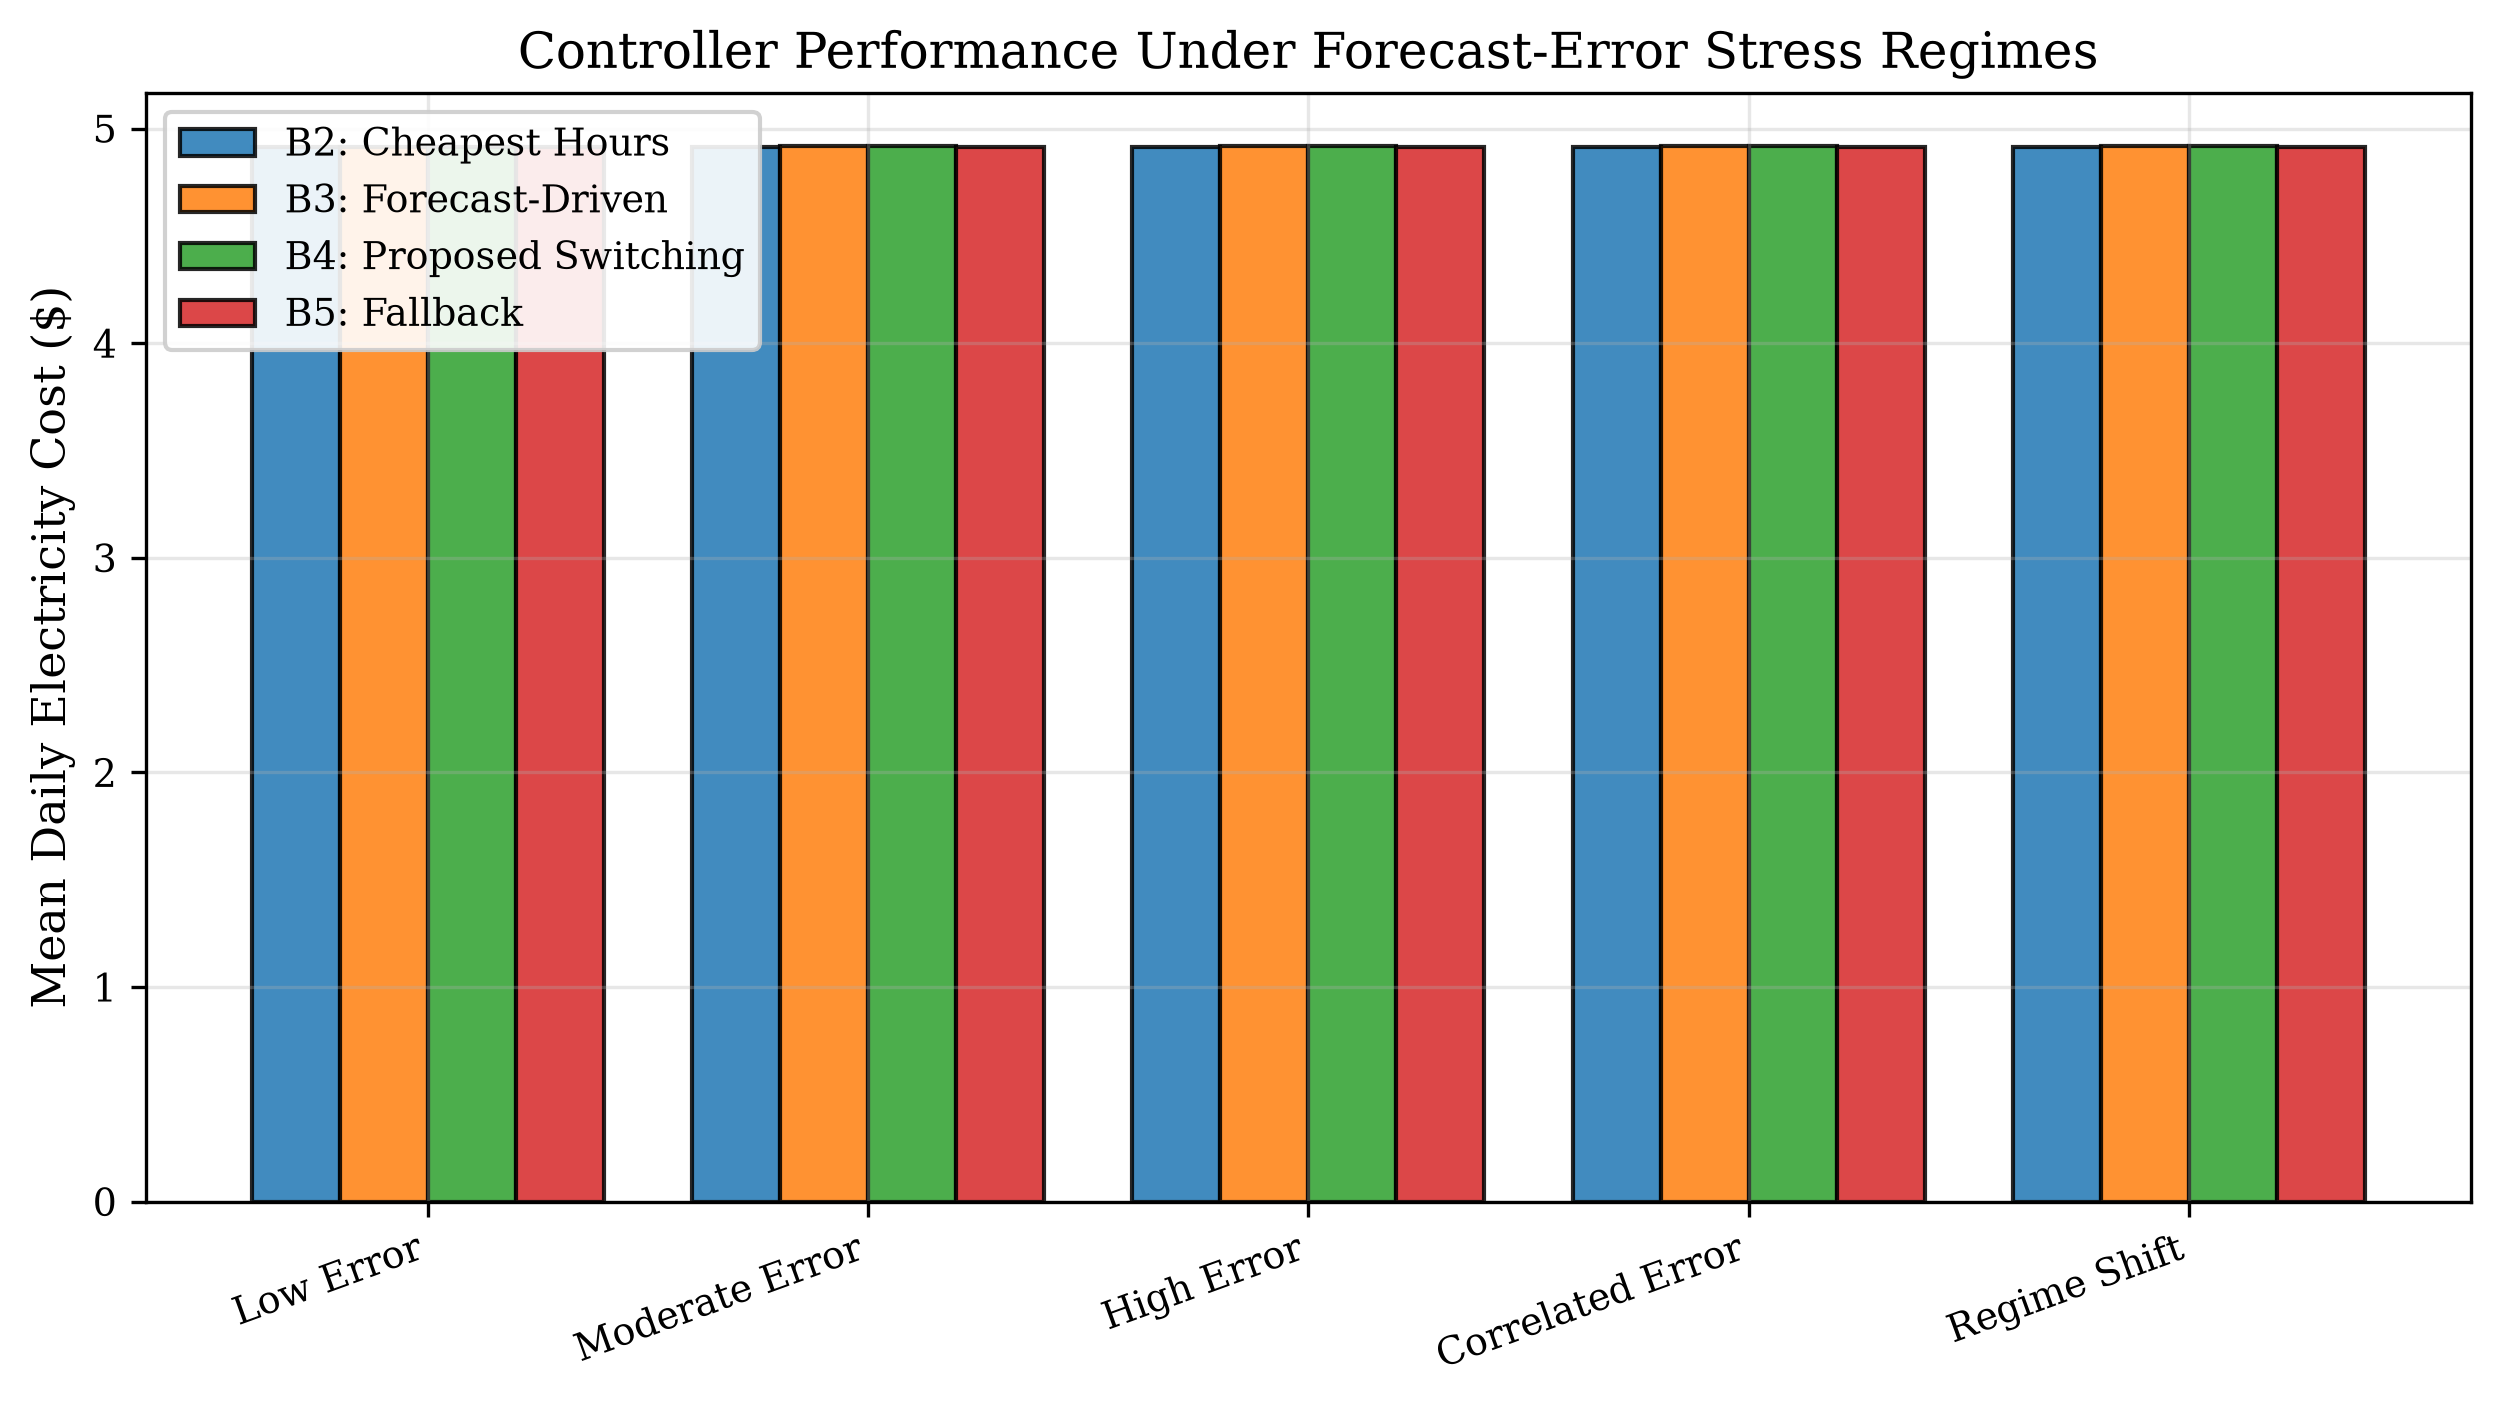
\includegraphics[width=0.49\textwidth]{fig8_stress_test_comparison.png}\hfill
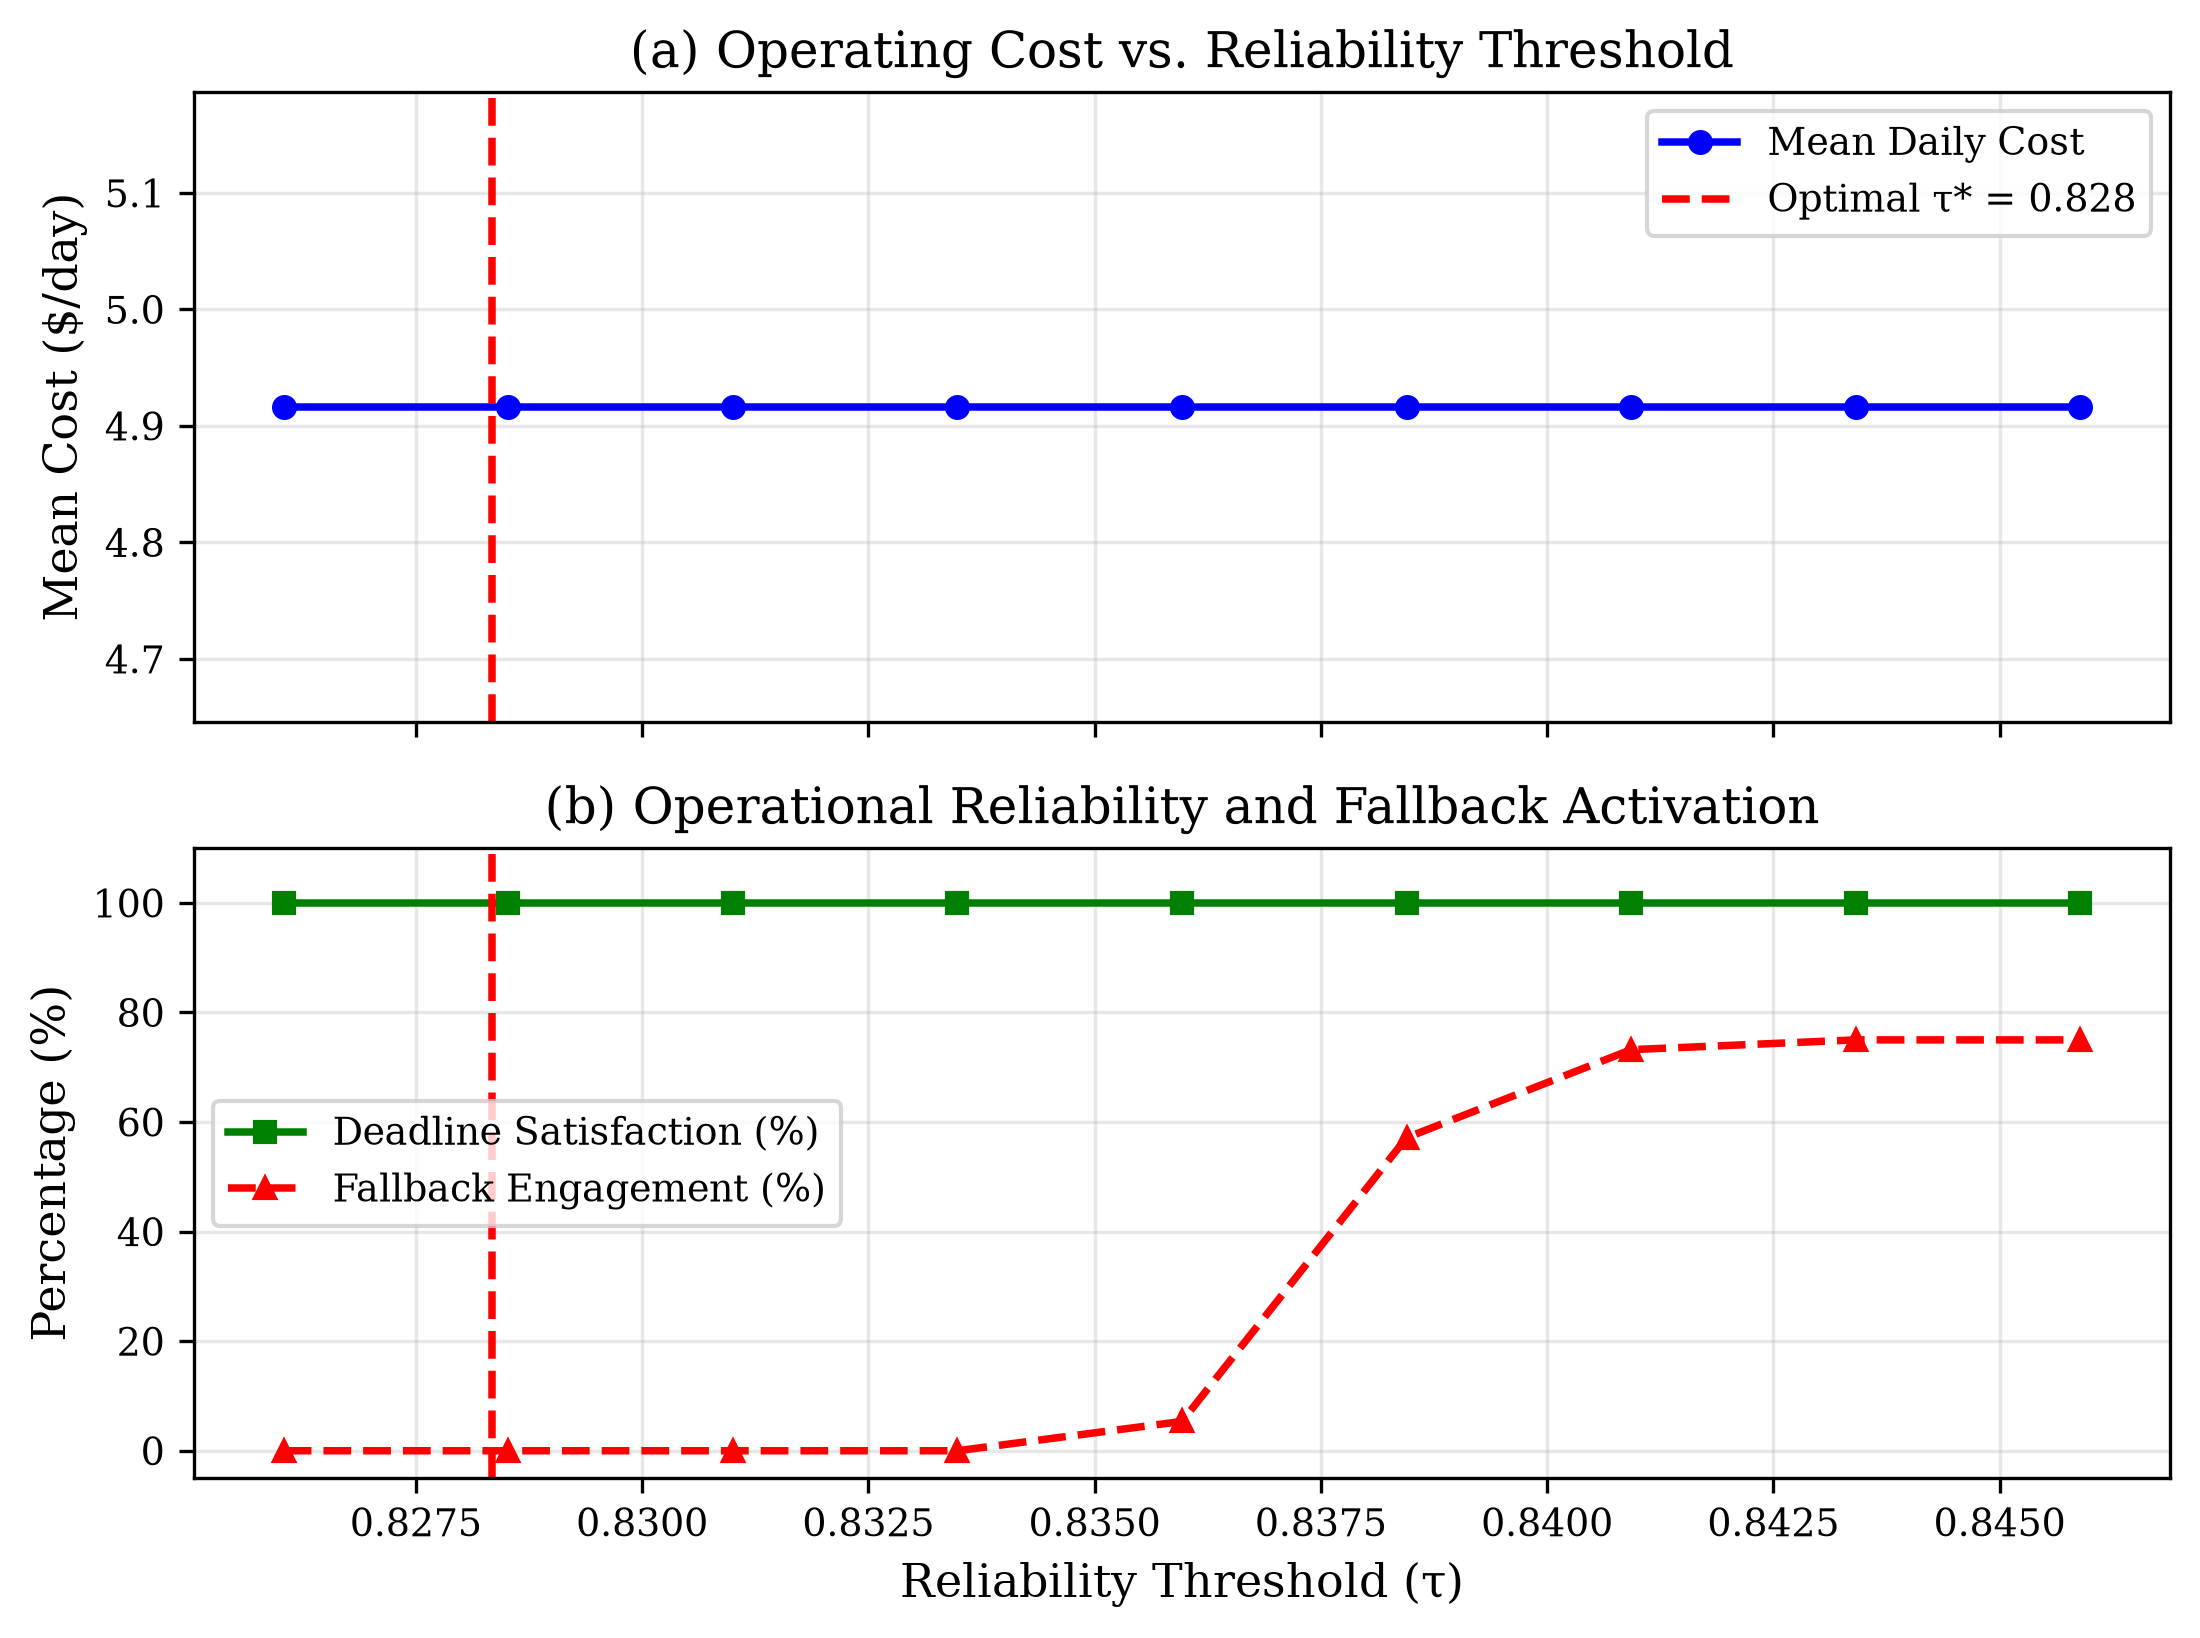
\includegraphics[width=0.49\textwidth]{fig9_threshold_sensitivity.png}
\caption{Left: controller performance under synthetic forecast-error stress regimes (low, moderate, high, correlated error, and cloud regime shift). Right: sensitivity of the reliability threshold $\tau$ on test days, showing (a) daily operating cost and (b) deadline satisfaction and fallback engagement rates.}
\label{fig:stress}
\end{figure*}

Under severe noise ($\sigma = 30\%$) and overcast regime shifts, the unconstrained forecast-driven scheduler (B3) suffered cost inflation (from \$4.9161 to \$4.9205/day), whereas the proposed switching controller (B4) engaged the fallback and preserved cost stability.

\section{Discussion}

\subsection{Evaluation of Research Hypotheses}
\begin{itemize}
    \item \textbf{H1 is supported}: All controllers achieved 100\% deadline satisfaction across all 56 test days and all stress regimes.
    \item \textbf{H2 is supported (weakly)}: Under nominal conditions, where forecast solar during connection hours is essentially zero, fallback and forecast-driven policies yield identical costs. Under severe stress, switching to the fallback insulates the home from forecast-induced deviations, although the observed cost difference is small (\$0.0044/day).
    \item \textbf{H3 is strongly supported}: For unidirectional charging, cheapest-hours charging (\$4.9161/day) outperforms solar-seeking policies. Since the vehicle arrives at 17:00 and departs at 07:00, solar generation is zero during 85\% of connection hours, and off-peak grid power at \$0.08/kWh is far cheaper than evening mid- or on-peak power (\$0.12--\$0.25/kWh).
    \item \textbf{H4 is strongly supported}: Bidirectional V2H flows deliver a statistically verified 26.4\% reduction in net daily cost (from \$4.5265 to \$3.3312/day). Discharging stored energy during the 17:00--21:00 on-peak period avoids purchases at \$0.25/kWh, while recharging occurs at \$0.08/kWh.
\end{itemize}

\subsection{Engineering and Policy Implications}
A practical insight for residential smart-charging design is that \textit{investing in complex solar-forecasting controllers for unidirectional EV charging yields negligible economic return if the connection window does not coincide with daytime solar hours.} When bidirectional V2H hardware is present, however, the vehicle acts as a stationary battery energy storage system, yielding major savings through diurnal tariff arbitrage while preserving mobility readiness.

\section{Limitations and Future Work}
This study is a numerical simulation on harmonized real-world data at hourly resolution. Limitations include: (i) no sub-hourly (e.g., 5-minute) irradiance ramp modeling, (ii) static battery degradation approximations, and (iii) no hardware-in-the-loop inverter validation. Future work will extend the framework to real-time receding-horizon model predictive control (MPC) on physical microgrid testbeds.

\section{Conclusion}
This paper presented a reproducible empirical investigation of reliability-aware residential EV charging using split conformal prediction and bidirectional V2H/V2G energy flows. Using measured solar PV, residential smart-meter demand, and a utility EV tariff, the proposed switching controller maintained 100\% deadline reliability while limiting forecast-error vulnerability. Bidirectional V2H flexibility further reduced daily electricity cost by 26.4\% through tariff arbitrage.

\balance
\bibliographystyle{IEEEtran}
\bibliography{references}

\end{document}